%%%%%%%%%%%%%%%%%%%%%%%%%%%%%%%%%%%%%%%%%%%%%%%%%%%%%%%%%%%%%%%%%%%%%%
% amspaper.tex --  LaTeX-based template for submissions to American 
% Meteorological Society journals
%
% Template developed by Amy Hendrickson, 2013, TeXnology Inc., 
% amyh@texnology.com, http://www.texnology.com
% following earlier work by Brian Papa, American Meteorological Society
%
% Email questions to latex@ametsoc.org.
%
%%%%%%%%%%%%%%%%%%%%%%%%%%%%%%%%%%%%%%%%%%%%%%%%%%%%%%%%%%%%%%%%%%%%%
% PREAMBLE
%%%%%%%%%%%%%%%%%%%%%%%%%%%%%%%%%%%%%%%%%%%%%%%%%%%%%%%%%%%%%%%%%%%%%

%% Start with one of the following:
% DOUBLE-SPACED VERSION FOR SUBMISSION TO THE AMS
\documentclass{ametsoc}

% TWO-COLUMN JOURNAL PAGE LAYOUT---FOR AUTHOR USE ONLY
% \documentclass[twocol]{ametsoc}

%%%%%%%%%%%%%%%%%%%%%%%%%%%%%%%%
%%% To be entered only if twocol option is used

\journal{jcli}

\usepackage{color}

%  Please choose a journal abbreviation to use above from the following list:
% 
%   jamc     (Journal of Applied Meteorology and Climatology)
%   jtech     (Journal of Atmospheric and Oceanic Technology)
%   jhm      (Journal of Hydrometeorology)
%   jpo     (Journal of Physical Oceanography)
%   jas      (Journal of Atmospheric Sciences)	
%   jcli      (Journal of Climate)
%   mwr      (Monthly Weather Review)
%   wcas      (Weather, Climate, and Society)
%   waf       (Weather and Forecasting)
%   bams (Bulletin of the American Meteorological Society)
%   ei    (Earth Interactions)

%%%%%%%%%%%%%%%%%%%%%%%%%%%%%%%%
%Citations should be of the form ``author year''  not ``author, year''
\bibpunct{(}{)}{;}{a}{}{,}

%%%%%%%%%%%%%%%%%%%%%%%%%%%%%%%%

%%% To be entered by author:

%% May use \\ to break lines in title:

\title{High-resolution regional climate model evaluation using variable-resolution CESM over California}

%change the title?

%%% Enter authors' names, as you see in this example:
%%% Use \correspondingauthor{} and \thanks{Current Affiliation:...}
%%% immediately following the appropriate author.
%%%
%%% Note that the \correspondingauthor{} command is NECESSARY.
%%% The \thanks{} commands are OPTIONAL.

    \authors{Xingying Huang, \correspondingauthor{Xingying Huang, 
     Department of Land, Air and Water Resources,
     University of California Davis, Davis, CA 95616.}
  Alan M. Rhoades and Paul A. Ullrich}

     \affiliation{Department of Land, Air and Water Resources, University of Califonia, Davis}

\email{xyhuang@ucdavis.edu}


    \extraauthor{Colin M. Zarzycki}
    \extraaffil{National Center for Atmospheric Research}


%%%%%%%%%%%%%%%%%%%%%%%%%%%%%%%%%%%%%%%%%%%%%%%%%%%%%%%%%%%%%%%%%%%%%
% ABSTRACT
%
% Enter your Abstract here

\abstract{Understanding the effect of climate change at regional scales remains a topic of intensive research. Computational constraints have meant that the high horizontal resolutions required to reach regional scales have been largely out of reach of modern global climate models. However, high horizontal resolution is needed to represent topographic forcing, which is a significant driver of local climate variability. Although regional climate models (RCMs) have traditionally been used at these scales, variable-resolution global climate models (VRGCMs) have recently arisen as an alternative for studying regional weather and climate. In this paper, the recently developed variable-resolution option within the Community Earth System Model (CESM) is assessed for long-term regional climate modeling. The mean climatology across California's diverse climate zones, including temperature and precipitation, is analyzed and contrasted with the Weather Research and Forcasting (WRF) model (as a traditional RCM), regional reanalysis, gridded observational datasets and uniform high-resolution CESM with the finite volume (FV) dynamical core. The results show that variable-resolution CESM is competitive in representing regional climatology on both annual and seasonal time scales. This assessment adds value to the use of VRGCMs for projecting climate change over the coming century and improve our understanding of both past and future regional climate related to fine-scale processes. This assessment is also relevant for addressing the scale limitation of current RCMs or VRGCMs when next-generation model resolution increases to $\sim$10km and beyond.} 

\begin{document}


%% Necessary!
\maketitle


%%%%%%%%%%%%%%%%%%%%%%%%%%%%%%%%%%%%%%%%%%%%%%%%%%%%%%%%%%%%%%%%%%%%%
% MAIN BODY OF PAPER
%%%%%%%%%%%%%%%%%%%%%%%%%%%%%%%%%%%%%%%%%%%%%%%%%%%%%%%%%%%%%%%%%%%%%
%
\section{Introduction}

Global climate models (GCMs) have been widely used to simulate both past and future climate. Although GCMs have demonstrated the capability to successfully represent large-scale features of the climate system, they are usually employed at coarse resolutions ($\sim$1$^\circ$), largely due to computational limitations. Global climate reanalysis datasets, which assimilate climate observations using a global model, represent a best estimate of historical weather patterns, but still have relatively low resolutions no finer than 0.5$^\circ$ (\url{http://reanalyses.org/atmosphere/overview-current-reanalyses}). Consequently, regional climate is not well captured by either GCMs or global reanalysis datasets.  However, dynamical processes at unrepresented scales are significant drivers for regional and local climate variability, especially over complex terrain \citep{soares2012wrf}. In order to capture these fine-scale dynamical features, high horizontal resolution is needed to allow for a more accurate representation of fine-scale forcings, processes and interactions \citep{leung2003regional, rauscher2010resolution}. We anticipate that with these enhancements the regional climate information will be more usable for policy makers and local stakeholders in formulating climate adaptation and mitigation strategies.

In order to model regional climate at high spatial and temporal resolution over a limited area, downscaling methods have been developed. There are largely two approaches for downscaling: The first is statistical downscaling, which aims to estimate fine scale behavior via analysis of the statistical relationships between observed small-scale variables and larger (GCM) scale variables \citep{fowler2007linking}. This method is empirical and cannot be used if the observed relationships do not hold with a changing climate \citep{soares2012wrf}. The second approach is dynamical downscaling, which uses a numerical model to simulate higher spatial resolution conditions in greater detail. Dynamical downscaling is popular and commonly employed using nested limited-area models (LAMs) to model regional scales \citep{laprise2008challenging}. In this context, LAMs are typically referred as regional climate models (RCMs) when applied to climate scales. RCMs are forced by output of GCMs or reanalysis data, and have been widely used, particularly to capture physically consistent regional and local circulations at the needed spatial and temporal scales \citep{christensen2007regional, bukovsky2009precipitation, mearns2012north}. Recently, variable-resolution global climate models (VRGCMs) have been increasingly employed for modeling regional climate. This approach uses a global model that includes high-resolution over a specific region and lower resolution over the remainder of the globe \citep{staniforth1978variable, fox1997finite}. VRGCMs have been demonstrated to be effective for regional climate studies and applications, owing to the advantages of traditional GCMs in representing large-scale features, at a reduced computational cost compared to uniform GCMs \citep{fox2001variable, fox2006variable, rauscher2013exploring, zarzycki2014using, zarzycki2014multidecadal, zarzycki2015localizedgrid}.

Compared with RCMs, a key advantage of VRGCMs is that they use a single, unified modeling framework, rather than a separate GCM and RCM. Thus, VRGCMs avoid potential inconsistency between the global and regional domains, and naturally support two-way interaction between these domains without the need for nudging \citep{warner1997tutorial, mcdonald2003transparent, laprise2008challenging, mesinger2013limited}. However, in order to obtain deeper insight into the performance of these two modeling approaches, it is necessary to compare them directly. For the purposes of this paper, we will focus on the recently developed variable-resolution Community Earth System Model (varres-CESM) as our VRGCM of interest. CESM is a state-of-the-art Earth modeling framework developed by the National Center for Atmospheric Research (NCAR), consisting of atmospheric, oceanic, land and sea ice components \citep{neale2010description}. Although CESM has been well-used for uniform resolution modeling, variable-resolution in the Community Atmosphere Model�s (CAM) Spectral Element (SE) dynamical core has only been recently developed and has yet to be rigorously investigated for long-term regional climate simulation \citep{taylor2010compatible, zarzycki2014using}. Consequently, the goal of this paper is to evaluate the performance of varres-CESM against gridded observational data, reanalysis data and in comparison to a dynamically downscaled modeling strategy.  Our variable-resolution simulations will focus on relatively high resolutions for climate assessment, namely 28km and 14km regional resolution, which are much more typical for dynamically downscaled studies.  For comparison with dynamical downscaling, the Weather Research and Forecasting (WRF) model will be used \citep{skamarock2005coauthors}. WRF has gained wide acceptance in studying regional climate over the past decade, showing its adequate capability in representation of fine-scale climate properties \citep{lo2008assessment, leung2009atmospheric, soares2012wrf}.  We anticipate that this assessment will add value in modeling mean regional climatology and improve our understanding about the effects of multi-scale processes in regional climate regulation. Our goal is also to advance the understanding of better use of models in future climate predictions and climatic extremes studies regionally.

%together with the traditional method of RCMs for the first time to see whether VRGCMs can show similar or even better ability in regional climate modeling. And simulations will be conducted at higher resolution than most former studies.  In this study, WRF (Weather Research and Forecasting)  For the VRGCM approach, 

Simulations using both varres-CESM and WRF have been performed for 26 years of historical climate with a regional domain centered on the state of California (CA). With its complex topography, coastal influences, and wide latitudinal range, this makes CA an excellent test bed for high-resolution climate studies. Also, an understanding of local climate variability is incredibly important for policymakers and stakeholders in California due to its vast agricultural industry, wide demographics, and vulnerability to anthropogenically-induced climate change \citep{hayhoe2004emissions, cayan2008overview}. RCM simulations over California have also been conducted in previous studies \citep{leung2004mid, kanamitsu2007fifty, caldwell2009evaluation, pan2011influences, pierce2013probabilistic}. \cite{caldwell2009evaluation}, in particular, presented results from WRF (Weather Research and Forecasting) at 12km spatial resolution showing both the overall consistency and some biases between simulations and observations.

This paper is organized as follows. Section 2 describes the model setup, evaluation methods and verification data. In section 3, results are demonstrated focusing on 2 m temperature (Ts) and precipitation (Pr). Key results are summarized along with further discussion in section 4.

%{\color{red} The introduction is too long?}

\section{Models and Methodology}

\subsection{Simulation design} 

All simulations use the AMIP (Atmospheric Model Intercomparison Project) protocols \citep{Gates1992}. AMIP simulations attempt to recreate a climatology similar to that observed over the past few decades. The ocean model is disabled and the model is forced with prescribed sea-surface temperatures (SSTs) and ice concentrations.

\subsubsection{WRF} 

The fully compressible non-hydrostatic WRF-ARW model in version 3.5.1 is used. ERA-Interim surface and pressure-level reanalysis was used to provide initial and lateral conditions for the domains. The lateral conditions and SSTs were updated every 6 hours. ERA-Interim reanalysis ($\sim$80 km) has been widely used and validated for its reliability as forcing data \citep{dee2011era}. Two simulations are conducted with horizontal resolution of 27km and 9km respectively, over the time period 1979-01-01 to 2005-12-31 (UTC). The year 1979 is used as a spin-up period and is discarded for purposes of analysis. The $\sim$10 km resolution is actually finer than most previous studies for long-term climate.

The simulation domains of WRF 9km are depicted in Figure \ref{fig:wrf_domains}. For the WRF 27km simulation, one domain is used.  For the WRF 9km simulation, two nested domains are used with the outer domain at 27km (same as the WRF 27km) and inner domain at 9km horizontal grid resolution. Two-way nesting is enabled.  These choices have been made to satisfy the natural WRF refinement ratio of 3:1.  Both grids are centered on CA and have respectively, 120$\times$110 and 151$\times$172 grid points. Around the boundaries, 10 grid points are used as lateral relaxation zones. In order to reduce the drift between forcing data and RCM, grid nudging \citep{stauffer1990use} was applied to the outer domain every 6 hours at all levels except the planetary boundary layer (PBL) as suggested by \cite{lo2008assessment}. This setup uses 41 vertical levels with model top pressure at 50 hPa.

%(check if other settings should add here): like topo, land cover, GHGs, aerosols

Additionally, we used the following physics parameterizations: WSM 6-class graupel microphysics scheme \citep{hong2006wrf}, Kain-Fritsch cumulus scheme \citep{kain2004kain}, CAM shortwave and longwave radiation schemes \citep{collins2004description}. These settings are supported by the one-year test running result with different options of cumulus scheme and radiation schemes. For the boundary layer, the Yonsei University scheme (YSU) \citep{hong2006new} and the Noah Land Surface Model \citep{chen2001coupling} were used. Both were chosen as they are common for climate applications that balance long-term reliability and computational cost.

\subsubsection{varres-CESM}

CESM has been under development for nearly two decades, and has been heavily used for understanding the effects of global climate change \citep{hurrell2013community}. Here, CAM version 5 (CAM5) \citep{CAM5Tech} and the Community Land Model (CLM) version 4 \citep{CLM40Tech} are used. As mentioned earlier, SE was used as the dynamical core in CAM along with the variable-resolution grid support. The FAMIPC5 compset was chosen for the simulations as it is the standard protocol for AMIP and is less computationally demanding. For our study, the variable-resolution cubed-sphere grids are generated for use in CAM and CLM with the open-source software package SQuadGen \citep{ullrich2014squadgen}. The grids used are depicted in Figure \ref{fig:varres-CESM_map}.  The maximum horizontal resolution on these grids are 0.25 degree ($\sim$ 28km) and 0.125 degree ($\sim$ 14km), with a 1 degree resolution covering the rest of the globe. These resolutions have been selected because CAM-SE naturally supports a 2:1 aspect ratio, meaning there are two transition layers from 1 degree to 0.25 degree, and one additional transition from 0.25 degree to 0.125 degree. As with the WRF simulations, the time period is from 1979-01-01 to 2005-12-31 (UTC), and year 1979 was discarded as spin up time for CLM4.0. Variable-resolution topography files have been produced by starting with the ETOPOV2 surface geopotential dataset and applying the differential smoothing technique outlined in \cite{zarzycki2015effects}. Land surface datasets, and plant functional types, were created at the standard 0.50 degree resolution. Greenhouse gas (GHG) concentrations are prescribed based on historical observations. SSTs and ice coverage are supplied by the 1degree Hadley Centre Sea Ice and Sea Surface Temperature dataset (HadISST) \citep{hurrell2008new}. Tuning parameters are not modified from their default configuration.

\subsection{Datasets}

Our evaluation focuses on near surface air temperature and precipitation, representative of the mean regional climate and climate variability on monthly, seasonal and annual time scales. For validation purpose, available reanalysis and gridded observational datasets of the highest quality are employed (see Table \ref{tab:Datasets}). These data products incorporate station measurements, satellite information and other observational data. Although these products are generally based on similar measurements, they are scaled and gridded using different techniques, causing processing uncertainty. Therefore, variation between these reference products represents observational uncertainty. We acknowledge that reanalysis products are particularly sensitive to model choice and choice of assimilated observations and so cannot be treated as truth. Our assessment focuses on the performance of the WRF and CESM simulations in terms of both mean behavior and variability. Detailed descriptions of these datasets are as follows.

% Due to the uncertainties in observations, we use different sources of datasets including measurements from stations, high-resolution reanalysis data or satellite information. 

\paragraph{NARR:}  The North American Regional Reanalysis (NARR) \citep{mesinger2006north} provides dynamically downscaled data over North America at $\sim$ 32 km resolution and 3 hourly intervals from 1979 through present. All major climatological variables are present in NARR, making it an excellent candidate for assessment of regional climate. Nonetheless, some inaccuracies have been identified in NARR that must be accounted for, including deficiencies in precipitation fields away from the continental US \citep{bukovsky2007brief}.

\paragraph{Daymet:}  Daymet is an extremely high resolution (1 km) gridded dataset with daily outputs of total precipitation, humidity, and minimum/maximum temperature covering the years of 1980 through 2013 \citep{thornton1997generating, thornton1999improved, thornton2000simultaneous}.  The dataset is produced using an algorithmic technique that ingests point station measurements in conjunction with a truncated Gaussian weighting filter.  Some adjustments are made to account for topography. Daymet is available through the Oak Ridge National Laboratory Distributed Active Archive Center (ORNL DAAC).

\paragraph{PRISM:}  The Parameter-elevation Regressions on Independent Slopes Model (PRISM) \citep{daly2008physiographically} supports a 4km gridded dataset obtained by taking point measurements and applying a weighted regression scheme that accounts for many factors affecting the local climatology.  The datasets include total precipitation and minimum, maximum and (derived) mean temperatures.  Monthly climatological variables are available for 1895 through 2014.  Daily data is available for the period 1981 through present, although the documentation is careful to state that since the observational input changes over time this data is not intended for multi-decadal trends.  This dataset will be used for detection and characterization of temperature and precipitation extremes.

\paragraph{UW:}  The UW daily gridded meteorological data is obtained from the Surface Water Modeling group at the University of Washington \citep{maurer2002long, hamlet2005production}. UW incorporated topographic corrections by forcing the long-term average precipitation to match that of the PRISM dataset. Temperature dataset is produced in a similar fashion as precipitation, but used a simple 6.1 K/km lapse rate for topographic effect.

%{\color{red}NLDAS?}

%The UW daily gridded meteorological data is obtained from the Surface Water Modeling group at the University of Washington \citep{maurer2002long}. The PRISM monthly gridded climate observations is produced by the PRISM (Parameter elevation Regression on Independent Slopes Model) Climate Group, and the dataset is based on a larger network of station data and accounts for elevation and topographic effects (cite??). UW Ts dataset is computed similarly to Pr, but without the topographic adjustment towards PRISM, and using a simple 6.1 K/km lapse rate. The Daymet gridded daily meteorological observations also take into account areas of complex terrain. The National Oceanic and Atmospheric Administration (NOAA) Climate Prediction Center (CPC) dataset uses more stations than the UW data, but without topographic correction (cite??). The National Centers for Environmental Prediction (NCEP) North American Regional Reanalysis (NARR) is NCEP's high resolution combined model and assimilated dataset (cite??).

\paragraph{Uniform CESM-FV:}  Output from a globally uniform CESM run at 0.25$^\circ$ global spatial resolution is utilized for comparison. This globally uniform simulation uses the CAM5-FV (finite volume) dynamical core and is described in additional detail in \cite{wehner2014resolution} and \cite{wehner2014effect}.  Note that the appendix of the latter paper lists parameters that are different from the public release.

%fvCAM5.1 
%1979-2005 observed SST, sea ice, CO2 and other greenhouse gases
%year 2000 climatology for the prescribed aerosols.

%Since the future simulations by RCMs can only be forced by GCM output, here, ~1 degree output of CESM is also used to force WRF to explore the effects of different boundary and initial conditions comparing with ERA-Interim. 

%{\color{red} These simulation use Need to ask Michael for a write-up of this dataset.}



\subsection{Post-processing}

For consistency, the reference datasets are averaged to the given model output resolution when differing and comparing statistical values such as root mean square error (RMSE), bias, and correlation. These datasets are remapped using a bilinear interpolation method, which has been verified to provide  satisfactory performance.  Other remapping algorithms, such as patch-based have been tested and do not exhibit notable differences.

%Bilinear interpolation is probably not the best technique; when the reference data is higher resolution than the model output you should average to a model grid cell. When the reference data is coarser resolution, it is usually not desirable to interpolate to a finer grid -- this does not take into account topographic features which can greatly affect the results. 

In order to better assess the treatment of specific climate regions, we divide the state into five regional zones, including: the Central Valley, Mountain Region, North Coast, South Coast, and Desert Region (Figure \ref{fig:wrf_domains}). For some parts of results analyses, simulations and datasets are masked to restrict climate variables to each region.

%{\color{red}not sure about capitalizing the sub-zones names}

\section{Results}

In this section, we assess the models' performances in terms of both temperature and precipitation over the 26 years period from 1980 to 2005. In particular, our comparison will focus on daily maximum, minimum and average 2m temperatures (Tmax, Tmin and Tavg), and daily precipitation (Pr), both annually and seasonally. These variables are key for a baseline climate assessment, particularly for their relationship with water resources, agriculture and health.

\subsection{Topography}

The grid-scale topography for all simulations is contrasted in Figure \ref{fig:topo}.  The higher resolution simulations provide a much finer representation of regional topography.  This is important for understanding local climate since topography is an important driver for fine-scale dynamic processes, especially over complex terrain.  Some differences are also apparent between the 28km varres-CESM and 27km WRF model, particularly over the Central Valley, and indicative of a different methodology for preparation of the topography dataset.  

%\subsection{Computational Cost}

%The simulations were run on a local server (Farm Cluster) at the University of California, Davis.  The daily throughput (real time/simulated day) for approximately 20 nodes (~480 processors) was 6.5 minutes for the varres-CESM 28 km run and 9.5 minutes for the varres-CESM 14km run. The WRF 27 km daily throughput was 2.5 minutes and the WRF 9 km was (INSERT HERE).

%The running time for a daily file is about 2 minutes and 25 minutes for WRF 27km and WRF 9km respectively.
%{\color{red}How many processors for each run?  More details on the cluster.}

 %{\color{red} for uniform CESM ?? -- no information available?}
 
 %Colin: I might not include this in the manuscript. We had some issues with CESM-SE not scaling properly on Agri (Infiniband problems and I/O bottlenecking) and I also did not tune it for maximum throughput (ex: I never bothered to get it working with OpenMP since I only get about a 10-15% speedup on Yellowstone with multiple threads). CAM-SE should run slower than WRF in a pure apples-to-apples sense, but I'm not sure that's a box we want to open up to reviewers without doing a more formal control study (or having many, many more simulations).

%{\color{red}computational cost part is masked here as Colin suggested}

\subsection{Temperature}

Here, daily maximum 2m temperature (Tmax), daily minimum 2m temperature (Tmin) and daily average 2m temperature (Tavg) from varres-CESM, WRF and the reference datasets over the simulation period are assessed.  We focus on the summer and winter seasons, representing June-July-August (JJA) and December-January-February (DJF). These periods are particularly relevant for local climate due to the impact of heat extremes during summer months and accumulation of snowpack during winter months.
%The annual average climatology of Tmax, Tmin and Tavg from varres-CESM, uniform CESM-FV, WRF and reference datasets over the simulation period are shown in Figures \ref{fig:Figure4}, \ref{fig:Figure5} and \ref{fig:Figure6}. Generally, simulations show similar regional patterns to observations, with a warmer central valley and southern deserts, colder northern coastal area and Sierra Nevadas mountain region. Both WRF and variable-resolution CESM demonstrate satisfactory {\color{red}(What is satisfactory?)} ability to model the annual climatology. Importantly, the higher resolution simulations perform better capturing fine features close to observations, especially for WRF 9km. 

The JJA Tmax and Tmin climatology are shown in Figures \ref{fig:t2max_JJA} and \ref{fig:t2min_JJA} respectively. For Tmax, generally all simulations show similar regional patterns to observations, but with a warm-biased in the Central Valley. Varres-CESM also shows a positive bias in the mountain region, especially at 0.25$^\circ$ resolution. On the contrary, WRF displays a cold bias outside of the Central Valley which is exacerbated with increased resolution. For Tmin, varres-CESM shows a larger bias than Tmax, with a particularly egregious overestimation of Tmin over Nevada (although errors are much smaller when focusing exclusively on California). WRF seems to better simulate Tmin with smaller bias than varres-CESM, with the sign of the bias dependent on individual climate zones. However, the pattern of Tmin present in Figure \ref{fig:t2min_JJA} in both WRF simulations suggests a cooler interior to the Central Valley and warmer perimeter, which is not supported by observations. Also note that errors are somewhat smaller when comparing with PRISM than with UW, so uncertainty among different observations must also be considered. Tavg (defined by averaging temperatures over one day) is also depicted in Figure \ref{fig:t2avg_JJA&DJF} (upper plots). Overestimation of Tmin by varres-CESM leads a similar overestimation for Tavg, although both models tend to have smaller biases in this case. The RMSE for these models over California range from 1 to 3$^\circ C$, as shown in Table \ref{tab:stat_JJA_t2}. RMSE and bias are calculated based on the 26-year average value of models and reference dataset over California. Overall, varres-CESM 0.125 degree performed the best in simulating long-term Tmax, whereas WRF 9km had the largest error. However, WRF is clearly better at modeling Tmin than varres-CESM. This is likely due, in part, to a positive 2 K SST bias near the California coastline, when comparing varres-CESM and WRF simulations. Examining biases, varres-CESM overestimated all JJA temperatures (especially Tmin), whereas WRF underestimates Tmax and Tavg and overestimates Tmin. When comparing against NARR (not shown), the biases for JJA Tmin and Tavg are largely reduced for varres-CESM. This suggests that the source of the temperature bias in varres-CESM and NARR may be related.

%Colin: Did we ever determine while the AMIP configurations for WRF and CESM are different? I could envision a picky reviewer harping on this. (for the 2 K SST bias)

The DJF climatology is discussed here primarily due to its impact on snowpack. For Tmax (Figure \ref{fig:t2max_DJF}), all simulations show a warm bias over the Central Valley (that is especially pronounced for WRF 27 km), but a cold bias over almost all other regions (particularly in the mountain region of the WRF 9km simulations). For Tmin (Figure \ref{fig:t2min_DJF}), the model simulations show a warm bias over most regions except the mountain region. These errors were evidently smaller when comparing to PRISM rather than UW. For Tavg (lower part of Figure \ref{fig:t2avg_JJA&DJF}), biases are quite smaller between models and PRISM dataset. Overall, the RMSEs are still roughly between 1 and 3 K, as noted in Table \ref{tab:stat_DJF_t2}, but were slightly reduced from summertime RMSEs. Simulations at coarser resolution seem to perform better overall, especially for varres-CESM 0.25$^\circ$ in Tmax, however, varres-CESM 0.25$^\circ$ shows largest error in modeling Tmin. For varres-CESM, biases were largely unaffected by moving to higher resolutions, with a slight underprediction of Tmax and pronounced overprediction of Tmin.  Moving to higher resolutions with WRF greatly increased biases in all cases.

Nevertheless, for both JJA and DJF climatology, spatial correlations are high between simulations and observations ($>$0.95), especially for Tmax and Tavg, and the error is relatively acceptable overall. This is especially encouraging since differences in the varres-CESM simulations, which only used prescribed SSTs, closely matched those of WRF, which were also forced at the lateral domain boundaries with reanalysis data.  In all cases, NARR exhibits obvious differences from other gridded observations, however uncertainty between the observational datasets is much smaller than the model biases, unlikely impacting our results. Also, the sea breeze effect, associated with cooler temperatures near the San Francisco Bay, are apparent in all runs. 

%The differences between model results and reference data are plotted in Figure \ref{fig:Figure7} for Tavg, highlighting some of the key differences between simulations, especially when considering individual climate zones.
 
%However, these models do exhibit some differences when examining different climate zones. In particular, Tmax is larger in the central valley in both CESM and WRF, and WRF 9km shows much more obvious cold bias in other regions than other simulations. Varres-CESM perform better than WRF and uniform CESM, especially at higher resolution. However, Tmin is obviously warmer by both WRF and CESM, especially at coastal region and southern desert, resulting under-prediction of diurnal range. WRF and uniform CESM perform better than varres-CESM. Varres-CESM and WRF perform similarly, better than uniform CESM. Comparing with PRISM, models show overall underestimation, especially at coastal and mountain regions, however with relatively small bias at most region. The RMSE for these models are basically ranges from 1 to 3 K, as showed by Table 2. Overall, variable-resolution CESM 0.125 deg performs best for long-term annual results, however,WRF 9km has larger error than WRF 27km. (varres-CESM > WRF > uniform CESM). And  Correlations are high between simulations and observations ($>$0.95), especially for Tmax and Tavg. There are about $+$2 K SST bias near the coast between varres-CESM and WRF. This may explain part of the reason for the above results. NARR shows obvious differences from other gridded observations, however, uncertainty between observational datasets are much smaller than the models' biases, unlikely impacting our results.

%For annual Tmax: Overestimate for WRF 9km. RMSE: CESM0.125<CESM 0.25<WRF27<WRF9<CESM uniform 0.25 around 1 to 3
%For annual Tmin: WRF 27<WRF9<CESM uniform<CESM 0.125<CESM 0.25 RMSE: similar around 1-3; Obviously overestimate, 
%For annual Tavg: Ranked from best to worst, we observe variable-resolution CESM 0.125 $>$ WRF 9km $>$ WRF 27km $>$ variable-resolution CESM 0.25 $>$ uniform CESM.

The seasonal cycle of Tavg is shown in Figure \ref{fig:trd_t2_allzones} for varres-CESM simulations, WRF simulations and reference data from PRISM and NARR. Monthly standard deviation is computed and are shown as vertical lines. The models do show good consistency with reference data and no larger than a 2$^\circ C$ bias, mainly in the coldest and hottest seasons. Comparing models, varres-CESM shows a smaller bias than WRF over the summer season everywhere except in the mountain region. However, WRF shows better performance in the winter season. In particular, varres-CESM and WRF show a cold bias in wintertime and summertime respectively compared with PRISM. Varres-CESM also shows a slightly larger year-to-year variability among seasons than observations as noted by the vertical lines, while WRF shows reduced variability. No significant differences can be discerned when comparing models across resolutions, although biases may be slightly larger at finer resolutions. Also, seasonal trends are similar among sub-zones, although exhibiting diverse magnitudes. Model performance appears to be worst in the coastal region and best in the desert and Central Valley.

%As for the multi-year monthly standard deviation, models are quite close to the reference dataset value of 4$^\circ$ -- except in the winter season, and especially at January, where varres-CESM and WRF 9km show about 1.5$\times$ and $2 \times$ larger standard deviation, respectively.

For the temperature climatology in California, we are more interested in the summer season, especially Tmax, due to the impact of summer heat extremes. We depict the frequency distribution of Tmax for the summer daily values, and compare the simulations to both Daymet and UW in Figure \ref{fig:PDF_t2max_allzones_JJA}. Properties of the Frequency distribution, including average, variability, skewness and Kurtosis are tabulated in Table \ref{tab:Table4}. Similar distribution shapes are present for both models and observations, although some mismatch occurs even between the observational datasets. Models are more close to each other, and more consistent with observations for higher values than the peak and less consistent at lower values. For representation of heat extremes, both varres-CESM and WRF 27km exhibit satisfactory performance over most regions except in Central Valley (CV). No obvious improvement is associated with higher resolution in varres-CESM. In the CV, the models show a clear warm bias and associated long tail, with temperatures reaching near 50$^\circ C$. As discussed above, all models do overestimate Tmax in the CV. In order to further assess the accuracy of the gridded observations, we examine the Tmax data directly from recorded weather station observations over the CV. The results validate that Tmax values above 45$^\circ C$ are rare (although station observations suggest these days may be slightly more frequent than suggested by UW and Daymet). The warm bias associated with the aforementioned extreme hot days in both varres-CESM and WRF is likely due to reasons discussed in \cite{caldwell2009evaluation} where biases were correlated with overly dry summertime soil moisture. This could be caused by insufficient physical parameterizations and the lack of accurate land surface treatment in climate models. Other reasons may include limited observations and unevenly distributed stations used to create the gridded datasets (i.e. interpolation bias).

%Former studies have already tried to alleviate this problem through parameterization (e.g. Liang et al. 2003; Yeh and Eltahir 2005; St�ckli et al. 2008) or through coupling with an explicit ground water model (e.g. York et al. 2005, Maxwell and Miller 2005; Maxwell et al. 2007). 

%since evaporation of soil moisture buffers daytime heating by solar radiation, variations in soil moisture have a stronger impact on daily maximum rather than daily minimum surface temperature. Insufficient subsurface water storage and lack of lateral flow are known sources of arid-season dry bias in RCMs and have been addressed in other studies As such, this study reaffirms the need for improved land surface treatment in climate models.
%the four moments

%{\color{red}[The gridded data show no instances of tempratures above 45$^\circ$ in the central valley.  Perhaps look back at weather station data to see if this is valid]} 

%Here, the annually average summer Tmax from models and reference data are displayed in Figures \ref{fig:Figure9} and \ref{fig:Figure10}. CESM generally overestimates Tmax especially for uniform CESM except at coastal region, while WRF showed obviously negative bias expect at central valley. Varres-CESM with higher resolution performed best as proved by the statistics in Table \ref{tab:Table3}, however, WRF 27km show less error than WRF 9km. Overall, models especially varres-CESM 0.125d and WRF 9km still show fairly accuracy over most regions.

%JJA Tmax: Variable resolution CESM with higher resolution performs better than at coarser resolution. RMSE 2 to 4; CESM 0.125<WRF9km<CESM 0.25<WRF27<CESM uniform; They have high correlations and the error is controlled between 1-2 Celsius. Overestimate for CESM, especially for uniform; underestimate for WRF;

\subsection{Precipitation}

Since the vast majority of California precipitation occurs in the winter season, only DJF precipitation will be assessed. The winter season is particularly important for California as it accounts for 50 percent of the 22.5 inches that California receives for its total annual average precipitation amounts (NOAA NCDC, 2014 - \url{http://www.ncdc.noaa.gov/cag/}).

The long-term average climatologies of DJF daily precipitation (Pr) from varres-CESM, WRF and reference datasets are displayed in Figure \ref{fig:pr_DJF}. Compared with observations, simulations do effectively capture regional patterns of precipitation. Precipitation is distributed mostly along the North coast and Sierra Nevada mountains, and is relatively sparse in other regions. However, there does exist clear differences among simulations. Varres-CESM overestimates total precipitation, especially in the coarse resolution (28 km) simulation along the western side of Sierra Nevada. The finer resolution simulation produces a slight reduction in that bias, likely due to improved treatment of orographic effects. Notably, there are large differences between WRF 27km and WRF 9km. WRF 27km underestimates total precipitation slightly, whereas WRF 9km shows a very large positive bias in total precipitation along the North coast and the Sierra Nevada of up to 50 percent. Overall, model performance was satisfactory, except for WRF 9km. Varres-CESM 0.125$^\circ$ performs slightly better than CESM 0.25$^\circ$ and WRF 27km, as further exhibited by the RMSE and bias values in Table \ref{tab:stat_Pr}. The observational datasets also have notable differences indicating uncertainty inherent in interpolating station data to a grid. However, these observations are still of the highest quality available and the uncertainty is relatively small compared with the simulations.


%The DJF precipitation from models and reference data as plotted in Figure \ref{fig:Figure12}. We can see that models and reference data show a similar pattern as annual precipitation, though the precipitations almost doubles in winter comparing with annual value {\color{red}You're averaging over a shorter period}.  Varres-CESM still overestimates total precipitation with larger absolute bias, especially at central valley {\color{red} (Possible reasons ??? -- Examine plots of PRECC and PRECL)}, and higher resolution still performs better. WRF 27km underestimates precipitation slightly, and WRF 9km still greatly overestimate in the North coastal region and the Sierra Nevada region. Considering the relatively heavy winter precipitation, the relative error is still acceptable for varres-CESM and WRF 27km, with RMSE and bias values showed in Table \ref{tab:Table4}.

%We can see that models and reference data show similar pattern as annual, though the precipitations almost doubles in winter comparing with annual value. varres-CESM still overestimate with larger absolute bias, especially at central valley {\color{red} (possible reasons ???)}, and higher resolution still performs better. WRF 27km underestimate a little, and WRF 9km still greatly overestimate at North coastal region and the sierra region. Considering the relatively heavy winter precipitation, the relative error is still acceptable for varres-CESM and WRF 27km, with RMSE and bias values showed in Table \ref{tab:Table4}.

%annual Pr: WRF 9km can be high as 12mm (1.5 times); CESM 0.125<CESM 0.25 and WRF 27<WRF 9.
%PRISM and Daymet are similar, so did not show PRISM here.
%plot the relative error??
%the reasons behind the large bias of WRF 9???
%add some percentage descriptions???

The climatological annual cycle of precipitation averaged over each sub-region is presented in Figure \ref{fig:trd_pr_allzones}. It can be seen that bias mainly occurs during the rainy seasons, especially in winter. WRF 27km is dryer in all regions and WRF 9km is far wetter in all regions. WRF 9km also shows larger variability compared with observations. Varres-CESM tracks well with observed precipitation everywhere except in the Central Valley, where precipitation is overestimated. It also exhibits a slightly larger variability in the rainy season than observations, while WRF 27km shows reduced variability. Nonetheless, the strong seasonal dependence on precipitation is apparent in all regions with extremely dry conditions during summer months.  A slight increase in summertime precipitation is apparent in the Desert region, indicative of the North American monsoon. Overall, varres-CESM is more consistent with observations in most regions and in all seasons compared with WRF, as can be seen in Table \ref{tab:Season_pr}. However, we also observe that the peak month for precipitation tends to occur earlier in varres-CESM than in observations. It is not surprising that a seasonal time drift occurred with the varres-CESM simulations as it was not forced by a reanalysis dataset (unlike the WRF simulations).

%{the plot of 26 years precipitation time trend}
%Caldwell: Description of temporal variability in the CCSM3 run is described in Bala et al. (2008). In particular, this simulation features a phase-locked ENSO with a period of 2 years.

The frequency distribution of wintertime Pr has been constructed from rainy days in winter (Pr$>$=0.1mm/d) and depicted in Figure \ref{fig:PDF_pr_allzones_DJF}. It can be seen that varres-CESM is more consistent with observations everywhere except in the CV. In this region WRF 27km appears to better capture high-intensity precipitation events, but performs more poorly on low-intensity events.  The underestimation of rainfall frequency in WRF 27km appears consistent across regions.  WRF 9km produces a significantly better treatment of low-intensity events, but greatly overestimates the frequency of high-intensity events.  Notably, varres-CESM 0.25 degree and varres-CESM 0.125 degree do not show significant differences. For strong precipitation events, varres-CESM and WRF 27km show satisfactory performance over most regions except in those noted above, although these conclusions are also constrained by observational uncertainty.

%This gives confidence for using varres-CESM in extreme precipitation studies. 

The positive bias of precipitation using WRF at high resolution has also been found in former studies. \cite{caldwell2009evaluation} gave a detailed discuss of possible reasons, stating that bias comes from a variety of source including the model itself and the choice of physical parameterizations.  A comprehensive analysis of the cause of these errors is beyond the scope of this paper. Further discussion can be found in former studies \citep{jankov2005impact, gallus2006comparison, chin2010preliminary, caldwell2010california}.

%DJF Pr: WRF 9km can be high as 24mm (also 1.5 times). For RMSE value is around one for CESM 0.125<WRF 27<CESM 0.25 <WRF 9 (around 4) 

%Figure convective precipitation VS micro-physics scheme especially for WRF 9km

Finally, a concise summary of model performance over CA is provided by the Taylor diagram (Figure \ref{fig:taylor_diagram}). This diagram includes the spatial correlation between the simulated and observed fields, the RMS variability of simulations normalized by that in the observations, and mean biases from reference data. It can be seen that the models correlate well with the PRISM reference dataset. Normalized standard deviation and bias are larger for precipitation, especially for WRF 9km. Varres-CESM performed better than WRF generally with essentially an opposite bias value in many cases. Overall, varres-CESM has demonstrated that it can competitively compare to WRF in capturing the regional climatology of California.

%At last, a concise summary of model performance annually over CA is provided by the Taylor diagram (Figure \ref{fig:Figure14}). This diagram includes the spatial correlation between the simulated and observed fields, the RMS variability of simulations normalized by that in the observations, and mean biases from verification data symboled at (1,0). It can be seen that models are close to reference data (PRISM), with small biases for temperature variables. Normalized standard deviation and bias are larger for precipitation, especialy for WRF 9km. varres-CESM performed better than WRF generally with opposite bias value in some cases. Overall, varres-CESM showed its comparable ability in studying high-resolution regional climatology against with regional climate model WRF.

%The angle between the x axis and the vector connecting the symbol and the origin indicates the spatial correlation between the simulated and ob- served fields. The distance from the origin indicates the RMS variability in the simulations normalized by that in the observations. Perfect agreement with verification data, with mean biases removed, would appear as a symbol plotted at (1, 0). Movement closer to (1, 0) between two simulations indicates improvement.


\subsection{varres-CESM and uniform CESM}

The climatological simulations for both varres-CESM 0.25$^\circ$ and uniform CESM-FV 0.25$^\circ$ are given in Figure \ref{fig:vr_uni_CESM} including Tmax, Tmin, Tavg and Pr. For JJA temperature, these two simulations show similar results. Differences are apparent in DJF temperature, where uniform CESM-FV exhibits smaller values than varres-CESM, leading to less bias over the Central Valley but larger bias over most other regions. For annual precipitation, compared with varres-CESM, uniform CESM-FV has less bias over central valley. However, uniform CESM-FV also overestimates Northern coast and mountain region precipitation in winter months. Overall, performance of varres-CESM was comparable to uniform CESM-FV.

%The climatology simulations of both varres-CESM 0.25 deg and uniform CESM-FV 0.25 deg are showed in Figure \ref{fig:Figure15} including Tmax, Tmin, Tavg and Pr. For JJA temperature, these two simulations show similar results. Differences are displayed in DJF temperature, uniform CESM showed smaller values than varres-CESM, which resulted less bias over central valley but larger bias over most other regions. For annual precipitation, comparing with varres-CESM, uniform CESM has obviously less bias over central valley. However, uniform CESM overestimated over part of northern coast and mountain regions in DJF Pr. In sum, Comparing with the uniform resolution CESM-FV simulation, varres-CESM performed similarly or even better in some cases.

\section{Discussions and summary}

This study has evaluated the performance of the relatively new varres-CESM against dynamically downscaled WRF and gridded reference datasets when simulating California climatology. As the need for assessments of regional climate change is increasing, alternative modeling strategies, including variable-resolution global climate models will be needed to improve our understanding of the effects of fine-scale processes in regional climate regulation. 

Based on 26 years of high-resolution historical climate simulation data over California, we analyzed both temperature and precipitation in California and across its climate divisions. We found that varres-CESM output performs slightly better than WRF for mean climatology, although the model still possessed slight biases towards a warmer and moister climate, especially in the Central Valley. WRF exhibited a clear cold bias in summer Tmax over most regions except the Central Valley, but an essentially opposite bias in summer Tmin, especially for the finer resolution simulation.  However, looking at the magnitude of RMSE, WRF was better overall at modeling Tmin. WRF also presented smaller daily temperature variability than both varres-CESM and the observational datasets. Higher resolution (0.125$^\circ$) simulations with varres-CESM were quite similar to the coarser resolution runs, although there were some improvements in capturing summer maximum temperature and precipitation. However, WRF 27km shows much better performance than WRF 9km, especially in modeling Tmax and precipitation trends. WRF 27km shows a slightly dryer climate, but WRF 9km dramatically overestimated precipitation over the North coastal region and the mountain region. Previous studies have also found this phenomenon for fine-scale simulations using RCMs as aforementioned. Additionally, we found that almost all of the precipitation comes from resolved (large-scale) processes for all these models, though convective scheme can also affect the large-scale microphysics results.

%and therefore we believe model biases are primarily associated with grid-scale dynamical processes rather than convective parameterizations.
%Colin: I wouldn't argue that the biases are being driven by purely the large-scale microphysics. A lot of work (i.e., Williamson) has shown that the partitioning of convective/large-scale is important. Ex: for tropical cyclones we see a high bias in precipitation that is partially mitigated by making the convective scheme more active by decreasing the relaxation timescale it operates on.

Models do show good consistency with reference data for seasonal Tavg, although varres-CESM exhibited a larger annual range in Tavg with colder winters and warmer summers. The main precipitation biases occured during rainy seasons, especially in winter. For describing the extreme hot events in summer, both varres-CESM and WRF 27km exhibit satisfactory performance over most regions except in Central Valley which may due to overly dry summertime soil moisture. For strong precipitation events, varres-CESM and WRF 27km show satisfactory modeling ability over most regions (except the Central Valley, in the case of varres-CESM), although the reference datasets also show some uncertainties. No obvious improvement is provided by moving from 28km to 14km resolution in varres-CESM.

Generally, when compared with observations, simulations do a good job of capturing regional climatological patterns. Spatial correlations are high between these simulations and observations. Errors are not indicative of deep underlying problems with the model formulation, but one should be aware of these biases when using these models for assessing future climate change. Uncertainty between observational datasets exists, but is much smaller than the models� biases. Compared with the uniform resolution CESM-FV simulation, varres-CESM performed similarly or even better in some cases. In summary, varres-CESM demonstrated competitive utility for studying high-resolution regional climatology when compared to a regional climate model (WRF) and a uniform high-resolution GCM (CESM-FV). This study suggests that variable-resolution GCMs are useful tools for assessing climate change over the coming century.

The importance and necessity of high resolution for regional climate studies has been widely stressed by previous studies. However, whether the current regional climate models can fulfill this demand when resolution is pushed to local scales is questionable. Based on our findings, WRF at 9km grid-scale produced larger biases than at 27km.  And further, varres-CESM at 14km resolution did not demonstrate clear improvement beyond 28km resolution. It is clear that further work is urgently needed to solve the scale limitation of current regional climate models at fine horizontal resolutions. The possible causes of the scale limitation may include a lack of accurate scare-aware physical parameterizations near or below 10 km horizontal resolution, the treatment of dynamics at fine scales, and the interactions among different components of RCMs or VR-GCMs (e.g., land-atmosphere interactions).

%In this way, VRGCMs can be expected to support longer simulations and incorporate more complicated physical parameter schemes. 
%In the future, even when a globally uniform simulation (at the highest resolution) becomes feasible to get the most accurate solution, regional high-resolution climate modeling can still be much more computationally feasible for very long simulations or simulations with extremely fine scales.

%SWE  Alan paper
%ensemble smooth: starting date???, the trd plot
%other seasons

%%%%%%%%%%%%%%%%%%%%%%%%%%%%%%%%%%%%%%%%%%%%%%%%%%%%%%%%%%%%%%%%%%%%%
% ACKNOWLEDGMENTS
%%%%%%%%%%%%%%%%%%%%%%%%%%%%%%%%%%%%%%%%%%%%%%%%%%%%%%%%%%%%%%%%%%%%%
\acknowledgments

The authors would like to thank Michael Wehner and Da\'ith\'i Stone for providing the uniform resolution CESM dataset. We would further like to thank Travis O'Brien for his many useful conversations on climate model assessment.  This project is supported in part by the University of California, Davis and by the Department of Energy ``Multiscale Methods for Accurate, Efficient, and Scale-Aware Models of the Earth System'' program.

 \bibliographystyle{ametsoc2014}
 \bibliography{database2015}

%\section{Figures and tables}

% TABLES

\begin{table}
\caption{Reanalysis and statistically downscaled observational datasets used in this study.} \label{tab:Datasets}
\begin{center}
\begin{tabular}{lcccc}
\hline \textbf{Data source} & \textbf{Variables used} & \textbf{Spatial resolution} & \textbf{Temporal resolution} \\
\hline \textbf{UW} & Pr, T$_{min}$, T$_{max}$ & 0.125$^\circ$ & daily \\
\textbf{PRISM} & Pr, T$_{min}$, T$_{max}$, T$_{avg}$ & 4km & monthly/daily \\
\textbf{DAYMET} & Pr, T$_{min}$, T$_{max}$ & 1km & daily \\
\textbf{NCEP CPC} & Pr & 0.125$^\circ$ & daily \\
\textbf{NARR} & Pr, T$_{s}$ & 32km & daily \\
\hline
\end{tabular}
\end{center}
\end{table}

%\begin{table}
%\begin{center}
%\caption{RMSE and Bias for annual temperature (California)} \label{tab:Table2}
%\begin{tabular}{lcccc}
%\hline \textbf{RMSE} & \textbf{UW}  & \textbf{PRISM} & \textbf{DAYMET} \\
%\hline $    $ & T$_{max}$ $\     $  T$_{min}$ & T$_{max}$ $\     $  T$_{min}$ $\     $ T$_{avg}$& T$_{max}$ $\     $  T$_{min}$\\
%\hline \textbf{Varres CESM 0.25d} & 1.605 $\     $ 3.035  & 2.098 $\     $ 2.393 $\     $ 1.753	&  2.109 $\     $ 3.170 \\
%\textbf{Varres CESM 0.125d} & 1.226 $\     $ 2.804  & 1.772	$\     $ 2.227	$\     $1.501 &	1.871 $\     $	2.884\\
%\textbf{Uniform CESM 0.25d} & 2.566 $\     $	2.558 &	2.949$\     $	2.437$\     $	2.418&	2.958$\     $	2.826 \\
%\textbf{WRF 27km} & 1.710	 $\      $ 2.506	 $\     $ & 2.240	 $\     $1.729 $\     $	1.721 &	2.105	 $\     $2.691 \\
%\textbf{WRF 9km} & 2.517	$\      $2.769&	2.732$\      $	1.764$\      $	1.420 & 2.581	$\      $ 2.752 \\
%\hline
%\end{tabular}

%\begin{tabular}{lcccc}
%\hline \textbf{BIAS} & \textbf{UW}  & \textbf{PRISM} & \textbf{DAYMET} \\
%\hline $    $ & T$_{max}$ $\     $  T$_{min}$ & T$_{max}$ $\     $  T$_{min}$ $\     $ T$_{avg}$& T$_{max}$ $\     $  T$_{min}$\\
%\hline \textbf{Varres CESM 0.25d} & -0.082$\     $	2.385 &	-0.353$\     $	1.296$\     $	-0.269 & 	-0.037 $\     $	2.256 \\
%\textbf{Varres CESM 0.125d} & -0.241$\     $	2.229	& -0.559$\     $	1.130$\     $	-0.438 &	-0.224	$\     $ 2.031\\
%\textbf{Uniform CESM 0.25d} & -0.409 $\     $	1.402	& -0.672	$\     $ 0.312	$\     $ -0.907	& -0.361$\     $	1.272 \\
%\textbf{WRF 27km} & -0.379$\     $	1.409 &	-0.649$\     $	0.321$\     $	-0.729 &	-0.336$\     $	1.282 \\
%\textbf{WRF 9km} & -1.805 $\     $	2.166 &	-2.123	$\     $ 1.067$\     $	-0.891	& -1.786$\     $	1.967 \\
%\hline
%\end{tabular}
%\end{center}
%\end{table}

%%%%%%%%%%%Table2%%%%%%%%%%%%%%%%%%%%%%%
\begin{table}
\begin{center}
\caption{RMSE and Bias for JJA temperature (California)} \label{tab:stat_JJA_t2}
\begin{tabular}{lcccc}
\hline \textbf{RMSE} & \textbf{UW}  & \textbf{PRISM} & \textbf{DAYMET} \\
\hline $    $ & T$_{max}$ $\     $  T$_{min}$ & T$_{max}$ $\     $  T$_{min}$ $\     $ T$_{avg}$& T$_{max}$ $\     $  T$_{min}$\\
\hline \textbf{varres-CESM 0.25d} & 2.324 $\     $ 3.752  & 2.932 $\     $ 3.136 $\     $ 2.614	&  2.810 $\     $ 3.938 \\
\textbf{varres-CESM 0.125d} & 1.903 $\     $ 3.639  & 2.452	$\     $ 2.961	$\     $2.195 &	2.477 $\     $	3.707\\					
%\textbf{Uniform CESM 0.25d} & 2.566 $\     $	2.558 &	2.949$\     $	2.437$\     $	2.418&	2.958$\     $	2.826 \\
\textbf{WRF 27km} & 2.311	 $\      $ 2.741	 $\     $ & 2.924	 $\     $2.252 $\     $	2.161 &	2.511	 $\     $2.993 \\
\textbf{WRF 9km} & 3.319	$\      $2.943&	3.470$\      $	1.847$\      $	1.752 & 3.203	$\      $ 2.945 \\
\hline
\end{tabular}

\begin{tabular}{lcccc}
\hline \textbf{BIAS} & \textbf{UW}  & \textbf{PRISM} & \textbf{DAYMET} \\
\hline $    $ & T$_{max}$ $\     $  T$_{min}$ & T$_{max}$ $\     $  T$_{min}$ $\     $ T$_{avg}$& T$_{max}$ $\     $  T$_{min}$\\
\hline \textbf{varres-CESM 0.25d} & 0.982$\     $	2.913 &	0.631$\     $	1.756$\     $	0.847 & 	1.177 $\     $	2.882 \\
\textbf{varres-CESM 0.125d} & 0.651$\     $	2.857	& 0.233$\     $	1.687$\     $	0.607 &	0.824	$\     $ 2.752\\				
%\textbf{Uniform CESM 0.25d} & -0.409 $\     $	1.402	& -0.672	$\     $ 0.312	$\     $ -0.907	& -0.361$\     $	1.272 \\
\textbf{WRF 27km} & -0.574$\     $	0.820 &	-0.925$\     $	-0.337$\     $	-0.747 &	-0.383$\     $	0.790 \\
\textbf{WRF 9km} & -2.274 $\     $	1.868 &	-2.693	$\     $ 0.698$\     $	-1.118	& -2.101$\     $	1.762 \\
\hline
\end{tabular}
\end{center}
\end{table}

%%%%%%%%Table3%%%%%%%%%%%%%%%%%%%%%%%%%
\begin{table}
\begin{center}
\caption{RMSE and Bias for DJF temperature (California)} \label{tab:stat_DJF_t2}
\begin{tabular}{lcccc}
\hline \textbf{RMSE} & \textbf{UW}  & \textbf{PRISM} & \textbf{DAYMET} \\
\hline $    $ & T$_{max}$ $\     $  T$_{min}$ & T$_{max}$ $\     $  T$_{min}$ $\     $ T$_{avg}$& T$_{max}$ $\     $  T$_{min}$\\
\hline \textbf{varres-CESM 0.25d} & 1.605 $\     $ 3.035  & 2.098 $\     $ 2.393 $\     $ 1.753	&  2.109 $\     $ 3.170 \\
\textbf{varres-CESM 0.125d} & 1.903 $\     $ 1.226  & 2.804	$\     $ 1.772	$\     $1.501 &	1.871 $\     $	2.884\\
%\textbf{Uniform CESM 0.25d} & 2.566 $\     $	2.558 &	2.949$\     $	2.437$\     $	2.418&	2.958$\     $	2.826 \\
\textbf{WRF 27km} & 1.710	 $\      $ 2.506	 $\     $ & 2.240	 $\     $1.729 $\     $	1.721 &	2.105	 $\     $2.691 \\
\textbf{WRF 9km} & 2.517	$\      $2.769&	2.732$\      $	1.764$\      $	1.420 & 2.581	$\      $ 2.752 \\
\hline
\end{tabular}

\begin{tabular}{lcccc}
\hline \textbf{BIAS} & \textbf{UW}  & \textbf{PRISM} & \textbf{DAYMET} \\
\hline $    $ & T$_{max}$ $\     $  T$_{min}$ & T$_{max}$ $\     $  T$_{min}$ $\     $ T$_{avg}$& T$_{max}$ $\     $  T$_{min}$\\
\hline \textbf{varres-CESM 0.25d} & -0.082$\     $	2.385 &	-0.353$\     $	1.296$\     $	-0.269 & 	-0.037 $\     $	2.256 \\
\textbf{varres-CESM 0.125d} & -0.241$\     $	2.229	& -0.559$\     $	1.130$\     $	-0.438 &	-0.224	$\     $ 2.031\\	
%\textbf{Uniform CESM 0.25d} & -0.409 $\     $	1.402	& -0.672	$\     $ 0.312	$\     $ -0.907	& -0.361$\     $	1.272 \\
\textbf{WRF 27km} & -0.379$\     $	1.409 &	-0.649$\     $	0.321$\     $	-0.729 &	-0.336$\     $	1.282 \\
\textbf{WRF 9km} & -1.805 $\     $	2.166 &	-2.123	$\     $ 1.067$\     $	-0.891	& -1.786$\     $	1.967 \\
\hline
\end{tabular}
\end{center}
\end{table}

%%%%%%%Table4%%%%%%%%%%%%%%%%%%%%%%%%%%%%%%

\begin{table}
\begin{center}
\caption{The first four moments of the JJA Tmax frequency in each sub-zone.  Column titles refer to Average (Avg), Variance (Var), Skewness (Skew) and Kurtosis (Kurt).} \label{tab:Table4}
\begin{tabular}{lccccc}
\hline \textbf{} & \textbf{Central valley}  & \textbf{Mountain} & \textbf{North coast} & \textbf{South coast} &\textbf{Desert}\\
\hline & Avg $\ $\ $ Var$\ $\ $Skew$\ $\ $ Kurt$ & Avg $\ $\ $ Var$\ $\ $Skew$\ $\ $ Kurt$  & Avg $\ $\ $ Var$\ $\ $Skew$\ $\ $ Kurt$  & Avg $\ $\ $ Var$\ $\ $Skew$\ $\ $ Kurt$  & Avg $\ $\ $ Var$\ $\ $Skew$\ $\ $ Kurt$  \\
%\hline \textbf{UW} &32.63$\ $	24.75	$\ $-0.77$\ $	0.91		& 26.68	$\ $33.17	$\ $-0.41$\ $	0.26&	25.92$\ $	 30.44	$\ $0.08	-0.51	&	25.92 $\ $ 30.44$\ $	0.08$\ $	-0.51 & 	37.01	$\ $ 22.87$\ $	-0.65 $\ $	0.68\\
%\textbf{Daymet} & 32.66	$\ $ 23.47$\ $ 	-0.86 $\ $ 	1.47	&	25.89$\ $ 	39.34	$\ $ -0.52	$\ $ 0.45	&	26.47	$\ $ 30.12	$\ $ -0.31	$\ $ 0.42		& 26.47	$\ $ 30.12	$\ $ -0.31$\ $ 	0.42	&	37.01	$\ $ 24.32	$\ $ -0.60	$\ $ 0.65\\
\hline \textbf{UW} &32.6$\ $	24.8	$\ $-0.8$\ $	0.9	&	26.7	$\ $33.2$\ $	-0.4	$\ $0.3	&	25.9	$\ $30.4	$\ $0.1$\ $	-0.5		&25.9$\ $	30.4	$\ $0.1$\ $	-0.5&		37.0	$\ $22.9$\ $	-0.6	$\ $0.7\\
\textbf{Daymet} & 32.7$\ $	23.5$\ $	-0.9$\ $	1.5	&	25.9	$\ $39.3$\ $	-0.5$\ $	0.5	&	26.5	$\ $30.1	$\ $-0.3$\ $	0.4	&	26.5	$\ $30.1	$\ $-0.3	$\ $0.4		& 37.0	$\ $24.3	$\ $-0.6$\ $	0.6\\
\hline\textbf{CESM 0.25d}& 34.1$\ $	26.2	$\ $-0.4$\ $	0.2	&	28.1	$\ $27.6$\ $	-0.4$\ $	0.3	&	26.4	$\ $37.4	$\ $0.1$\ $	-0.7		& 26.4$\ $	37.4	$\ $0.1$\ $	-0.7	&	37.6$\ $	19.0$\ $	-0.5	$\ $0.8\\
\textbf{CESM 0.125d}& 34.3	$\ $28.5$\ $	-0.5	$\ $0.4	&	27.2	$\ $30.0$\ $	-0.4$\ $	0.3	&	26.3	$\ $37.4$\ $	0.1$\ $	-0.6		& 26.3$\ $	37.4$\ $	0.1	$\ $-0.6		& 37.3	$\ $21.3$\ $	-0.5	$\ $0.4\\
\hline\textbf{WRF 27km} & 33.9	$\ $34.8	$\ $-0.5$\ $	0.2	&	24.9	$\ $34.8$\ $	-0.3	$\ $0.0	&	26.0	$\ $36.7	$\ $-0.1$\ $	-0.5		& 26.0$\ $	36.7	$\ $-0.1	$\ $-0.5		& 36.5$\ $	22.6$\ $	-0.6$\ $	0.5\\
\textbf{WRF 9km}&32.4		$\ $33.1	$\ $	-0.7	$\ $	0.6	&	22.4		$\ $38.5		$\ $-0.5		$\ $0.6	&	24.9	$\ $	32.6		$\ $0.0		$\ $-0.6	&	24.9	$\ $	32.6	$\ $	0.0		$\ $-0.6	&	34.4		$\ $24.4		$\ $-0.5		$\ $0.4\\
\hline
\end{tabular}
\end{center}
\begin{tabular}{p{6in}}
\textbf{Notes:} If skew $>0$ [skew $<0$], the distribution trails off to the right [left]. If kurtosis $> 0$ [$<0$], it is usually more sharply peaked [flatter] than the normal distribution (leptokurtic and platykurtic, respectively).
%E.g., a rectangular function has a kurtosis of -1.2 (=1.8-3) relative to the normal distribution.
\end{tabular}
\end{table}
%If skew>0 [skew<0], the distribution trails off to the right [left].
%If kurtosis > 0 [<0], it is usually more sharply peaked [flatter] than the normal distribution (leptokurtic and platykurtic, respectively). E.g., a rectangular function has a kurtosis of -1.2 (=1.8-3) relative to the normal distribution.
%average variance skewness kurtosis

%%%%%%Table5%%%%%%%%%%%%%%%%%%%%%%%%%%%

\begin{table}
\begin{center}
\caption{RMSE and Bias for Precipitation (California)} \label{tab:stat_Pr}
\begin{tabular}{lcccc}
\hline \textbf{Annual} & \textbf{CPC}  & \textbf{UW} & \textbf{PRISM} & \textbf{DAYMET} \\
\hline $    $ & RMSE $\     $  Bias & RMSE $\     $  Bias & RMSE $\     $  Bias & RMSE $\     $  Bias \\
\hline \textbf{varres-CESM 0.25d} & 0.590	$\     $ 0.370 &	0.604 $\     $	0.265 &	0.726	$\     $ 0.171 &	0.560$\     $	0.169 \\
\textbf{varres-CESM 0.125d} &0.481 $\     $ 	0.220 &	0.534 	$\     $ 	0.126 &	0.634 $\     $  0.050	& 0.510	$\     $  0.043\\
%\textbf{uniform CESM 0.25d} & 0.551$\     $	0.118 &	0.601 $\     $	0.012 &	0.708$\     $	-0.082	& 0.603 $\     $	-0.083 \\
\textbf{WRF 27km} & 0.424$\     $	-0.210 &	0.586$\     $	-0.315 &	0.777$\     $	-0.409 &	0.650$\     $	-0.411 \\
\textbf{WRF 9km} & 2.204	 $\     $ 1.462 &	2.026$\     $	1.368	& 1.858 $\     $	1.292 &	1.986 $\     $	1.286\\
\hline
\end{tabular}

\begin{tabular}{lcccc}
\hline \textbf{DJF} & \textbf{CPC}  & \textbf{UW} & \textbf{PRISM} & \textbf{DAYMET} \\
\hline $    $ & RMSE $\     $  Bias & RMSE $\     $  Bias & RMSE $\     $  Bias & RMSE $\     $  Bias \\
\hline \textbf{varres-CESM 0.25d} & 1.409	$\     $ 0.883	& 1.401	$\     $ 0.558	& 1.636 $\     $	0.465	& 1.310 $\     $	0.404 \\
\textbf{varres-CESM 0.125d} &1.236	$\     $ 0.666 &	1.273	$\     $  0.362 &	1.436 $\     $ 	0.307 &	1.210 $\     $ 	0.234\\
%\textbf{uniform CESM 0.25d} & 1.353 $\     $	0.273	& 1.440$\     $	-0.052	& 1.566	$\     $ -0.146	& 1.419	$\     $ -0.206 \\
\textbf{WRF 27km} &0.918 $\     $	-0.396 &	1.331  $\     $	-0.721	& 1.588  $\     $	-0.815 &	1.389	 $\     $ -0.876 \\
\textbf{WRF 9km} & 4.244 $\     $2.562	& 3.801	$\     $ 2.257 &	3.538$\     $	2.203 &	3.782	$\     $ 2.132\\
\hline
\end{tabular}
\end{center}
\end{table}

%%%%%%%%%%%Table6%%%%%%%%%%%%%

\begin{table}
\begin{center}
\caption{Seasonal Average Precipitation for five sub-divisions of California} \label{tab:Season_pr}
\begin{tabular}{lcccc}
\hline \textbf{} & \textbf{SON}  & \textbf{DJF} & \textbf{MAM} & \textbf{JJA} \\
\hline & CV $\ $\ $\  $Mt$\ $\ $\  $NC$\ $\ $\ $SC$\ $\ $\ $Dt& CV $\ $\ $\  $Mt$\ $\ $\  $NC$\ $\ $\ $SC$\ $\ $\ $Dt& CV $\ $\ $\  $Mt$\ $\ $\  $NC$\ $\ $\ $SC$\ $\ $\ $Dt & CV $\ $\ $\  $Mt$\ $\ $\  $NC$\ $\ $\ $SC$\ $\ $\ $Dt\\
\hline \textbf{UW} $    $& 1.14	$\ $1.68  $\ 1.92$\ 0.59 $\ $ 0.31 & 3.62$\ $ 4.31 $\ 6.19 $\ 2.75$\ $ 0.89 & 1.72$\  $	2.22$\  $2.64$\  $1.16$\  $	0.38 &0.13	$\  $	0.41$\  $		0.18$\  $		0.07$\  $		0.22\\
\textbf{PRISM}&1.21$\  $	1.82$\  $	2.17$\  $	0.64	$\  $0.31 &3.49$\  $	4.50	$\  $6.39$\  $	2.93	$\  $0.89& 1.75	$\  $2.38	$\  $2.84$\  $	1.25$\  $	0.39 & 0.14	$\  $0.46$\  $	0.22$\  $	0.05$\  $	0.25\\
\hline\textbf{CESM 0.25d}&1.89	$\  $1.90$\  $	2.20$\  $	0.57$\  $	0.42		&	5.35	$\  $4.62$\  $	5.87$\  $	2.87	$\  $1.27	&		2.35	$\  $2.35	$\  $2.56$\  $	0.83	$\  $0.48	&		0.10$\  $	0.47	$\  $0.13$\  $	0.07	$\  $0.20\\
\textbf{CESM 0.125d}& 1.22	$\  $1.45$\  $	1.72$\  $	0.42	$\  $0.40		&	4.95$\  $	4.46$\  $	5.82	$\  $2.70	$\  $1.09		&	2.32$\  $	2.46	$\  $2.51$\  $	1.09	$\  $0.48		&	0.10	$\  $0.50$\  $0.13$\  $	0.06	$\  $0.22
\\
\hline\textbf{WRF 27km}& 0.87	$\  $1.33	$\  $1.30$\  $	0.46$\  $	0.20		&	3.05$\  $	3.86	$\  $4.18	$\  $1.97$\  $	0.47		&	1.44	$\  $2.12$\  $	1.84	$\  $0.94	$\  $0.20		&	0.10	$\  $0.57	$\  $0.21	$\  $0.10$\  $	0.08
\\
\textbf{WRF 9km}&2.13$\  $	3.69	$\  $3.35$\  $	1.20$\  $	0.97	&		5.74$\  $	8.26$\  $	8.84	$\  $4.10	$\  $1.08		&	3.05	$\  $4.38$\  $	4.18	$\  $1.71	$\  $0.49		&	0.32	$\  $1.78$\  $	0.43$\  $	0.24$\  $	0.80	\\		    		
\hline 									 
\end{tabular}
\begin{tabular}{p{6in}}
\textbf{Notes:}  SON (September-October-November), DJF (December-January-February), MAM (March-April-May), JJA (June-July-August); CV (central valley), Mt (Mountain), NC (North coast), SC (South coast), Dt (Desert).
\end{tabular}
\end{center}
\end{table}

%(SON (September-October-November), MAM (March-April-May), CV (central valley)  Mt (Mountain)  NC (North coast)  SC (South coast)  Dt (Desert) )	

%\subsection{Figures}

\begin{figure}
\begin{center}
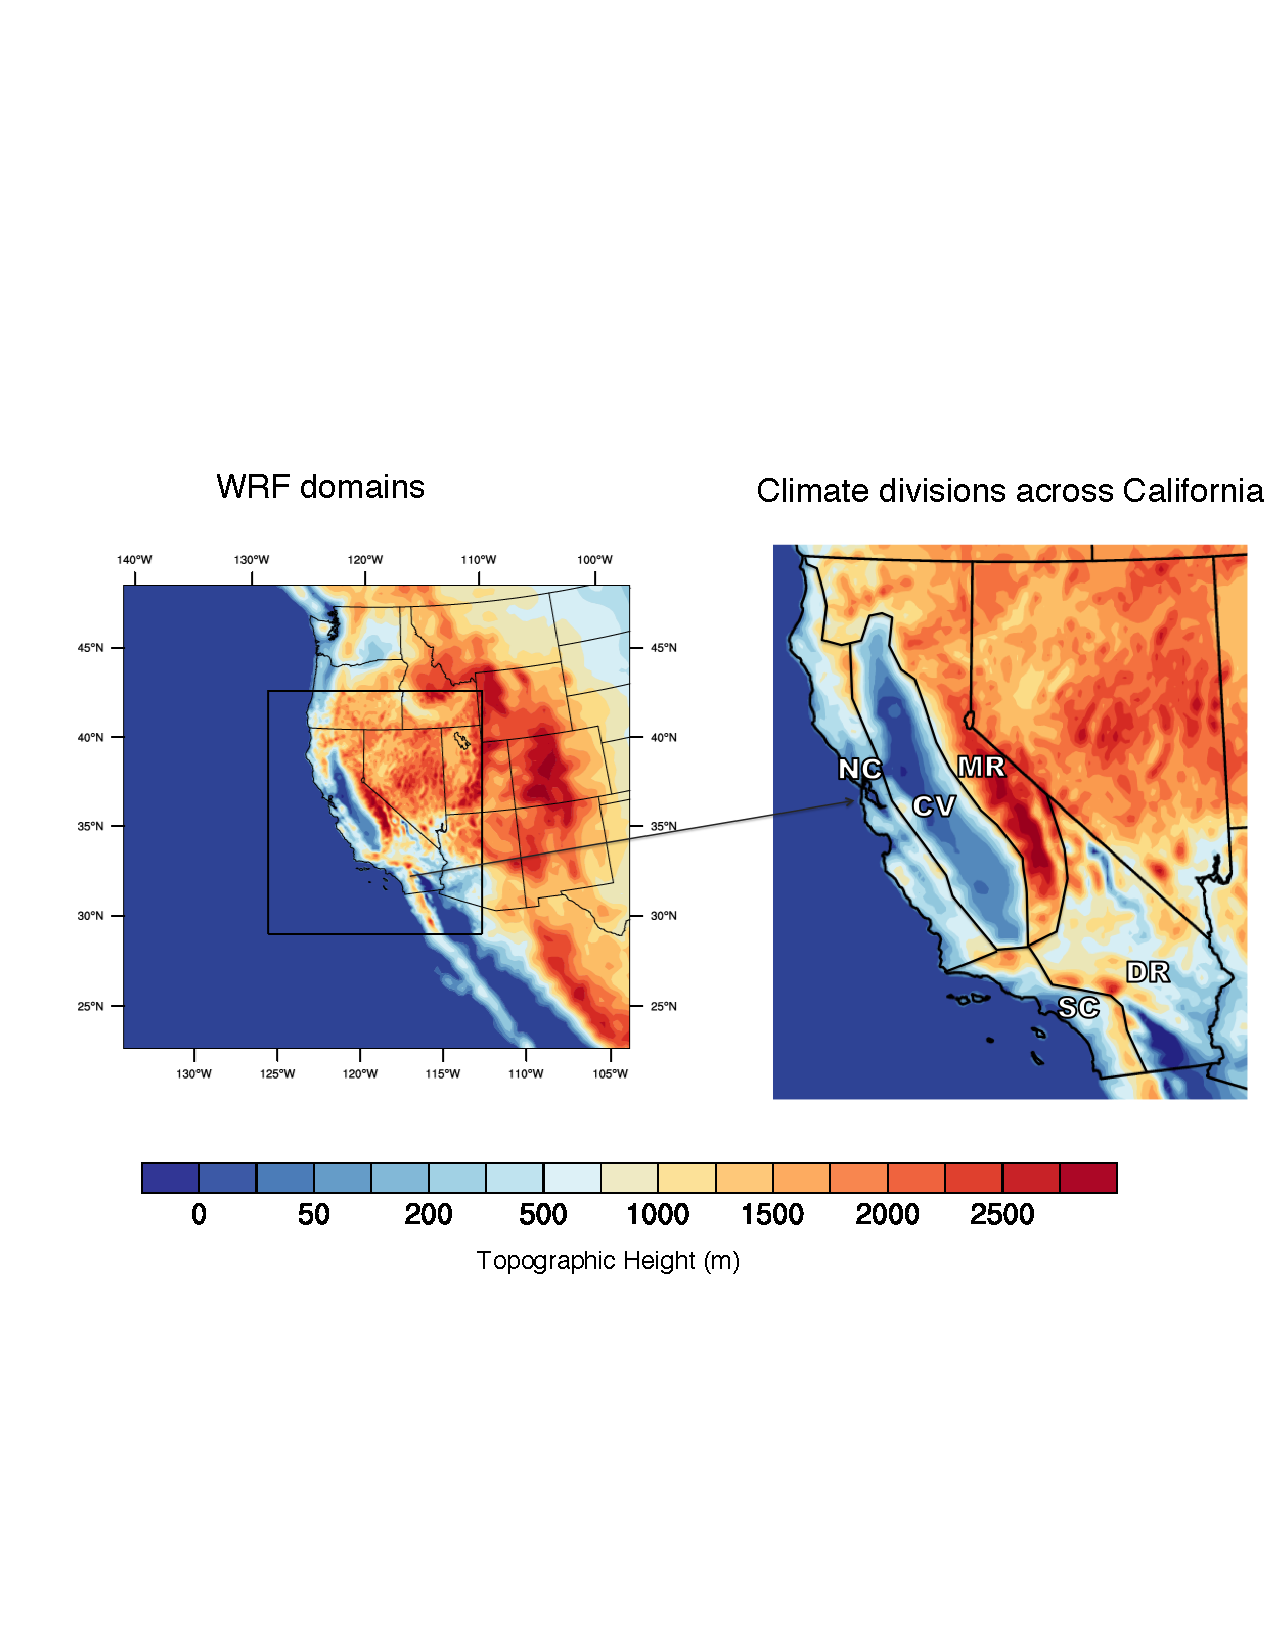
\includegraphics[width=6in]{wrf_domains.pdf}
\end{center}
\caption{Domains of WRF simulations (left) and five climate divisions in California (right) with topography in meters (m). } \label{fig:wrf_domains}
\end{figure}

\begin{figure}
\begin{center}
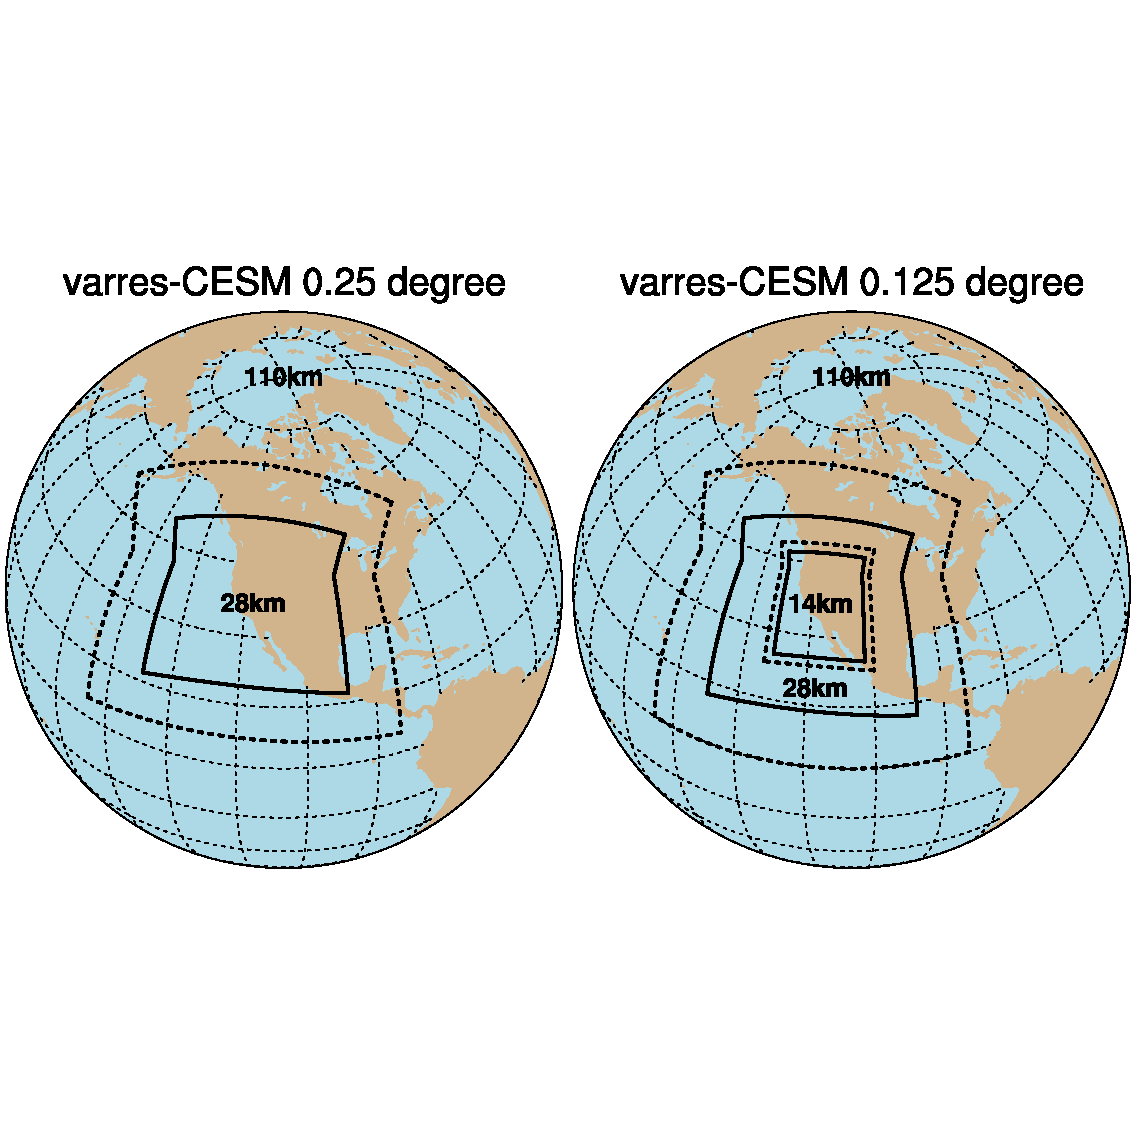
\includegraphics[width=6in]{varres-CESM_map}
\end{center}
\caption{Approximate regional resolution for the computational grids used in varres-CESM simulations.  The dashed lines and solid lines correspond to the outer boundary and inner boundary of the transition region.} \label{fig:varres-CESM_map}
\end{figure}

\begin{figure}
\begin{center}
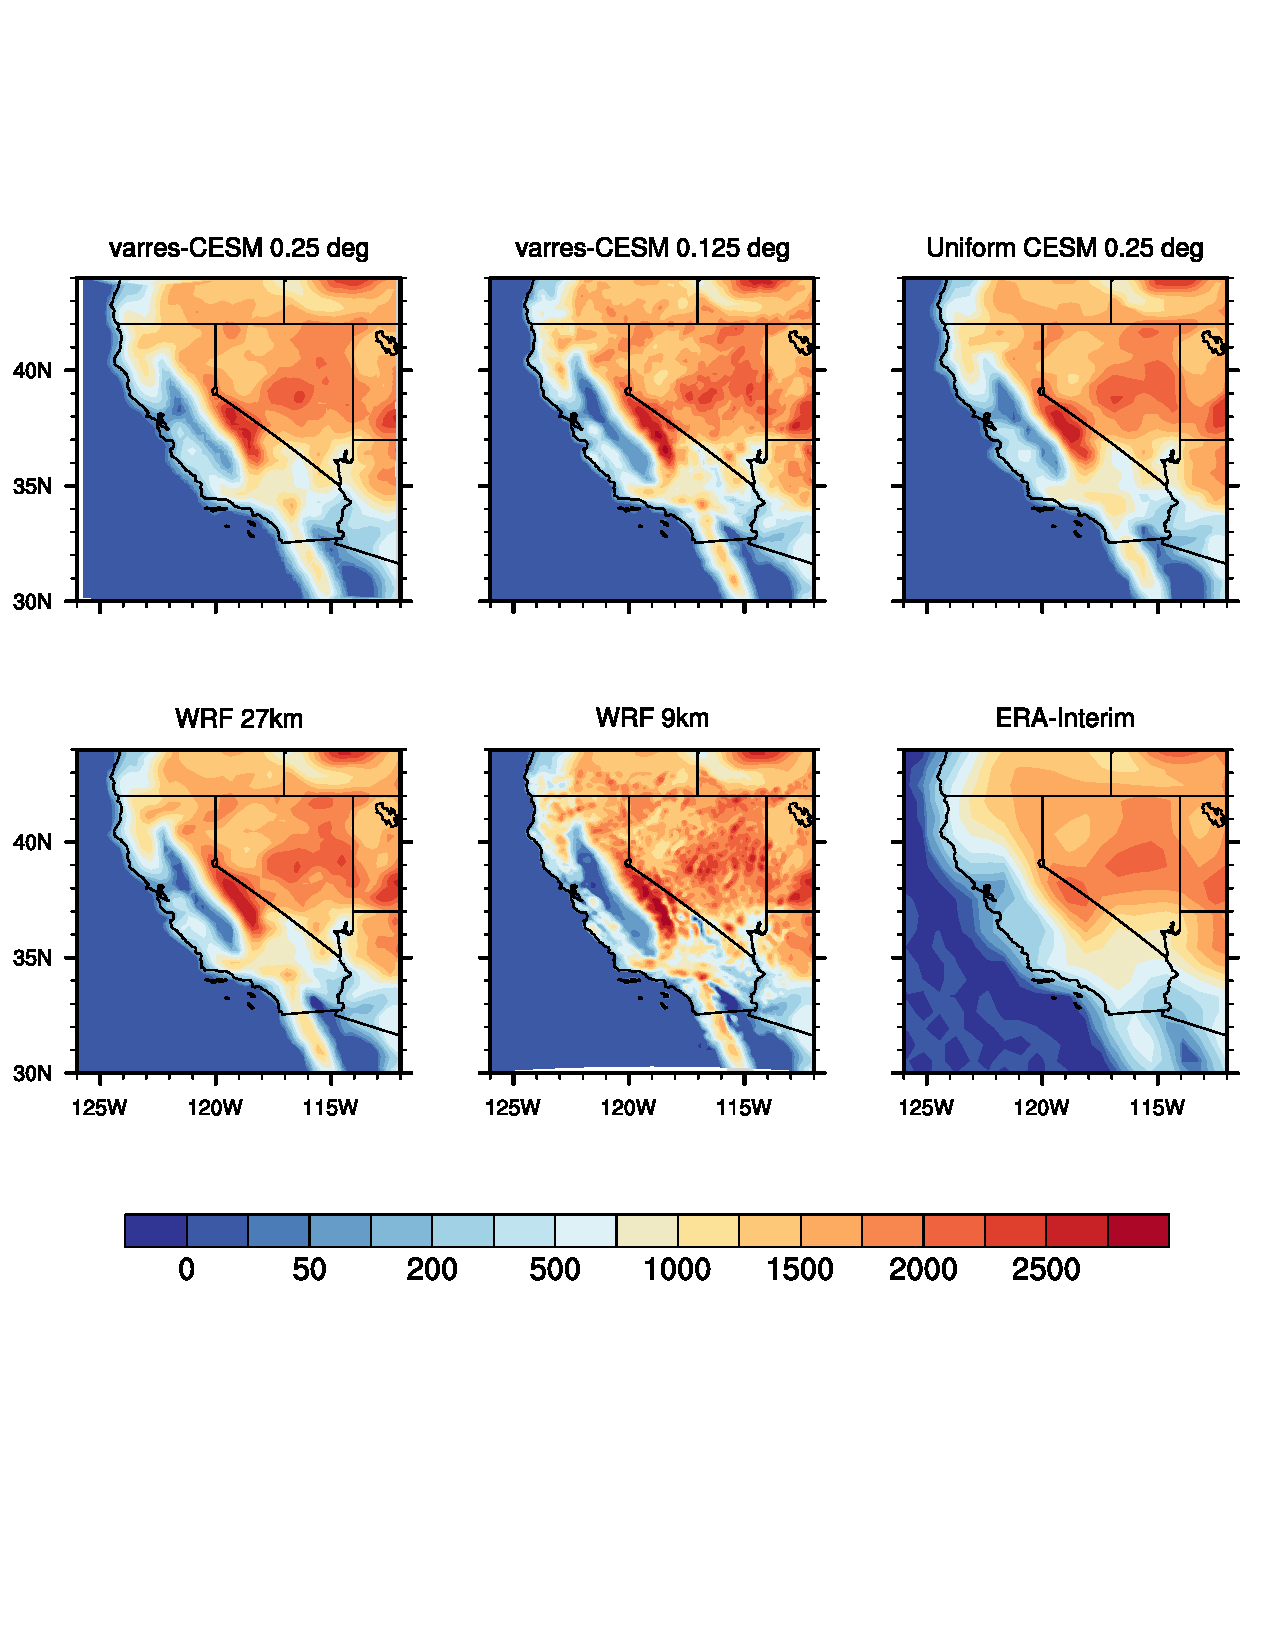
\includegraphics[width=6in]{topo.pdf}
\end{center}
\caption{Topography in meters (m) for (top left to bottom right) varres-CESM 0.25$^\circ$, varres-CESM 0.125$^\circ$, uniform CESM-FV 0.25$^\circ$, WRF 27km, WRF 9km and ERA-Interim ($\sim$80 km).} \label{fig:topo} 
\end{figure}

\begin{figure}
\begin{center}
\includegraphics[width=6in]{t2max_JJA.pdf}
\end{center}
\caption{JJA average daily Tmax from models and reference datasets, and differences between them ($^\circ$C).            
(Daymet is similar to PRISM, and so isn't shown in the difference plot).} \label{fig:t2max_JJA}
\end{figure}

\begin{figure}
\begin{center}
\includegraphics[width=6in]{t2min_JJA.pdf}
\end{center}
\caption{As Figure 4, but for summer Tmin. 
(Daymet is similar to UW, so not shown in difference plot)} \label{fig:t2min_JJA}
\end{figure}

\begin{figure}
\begin{center}
\includegraphics[width=6in]{t2avg_JJA&DJF.pdf}
\end{center}
\caption{As Figure 4, but for Tavg in JJA and DJF.} \label{fig:t2avg_JJA&DJF}
\end{figure}

\begin{figure}
\begin{center}
\includegraphics[width=6in]{t2max_DJF.pdf}
\end{center}
\caption{As Figure 4, but for winter Tmax.} \label{fig:t2max_DJF}
\end{figure}

\begin{figure}
\begin{center}
\includegraphics[width=6in]{t2min_DJF.pdf}
\end{center}
\caption{As Figure 4, but for winter Tmin.} \label{fig:t2min_DJF} 
\end{figure}


\begin{figure}
\begin{center}
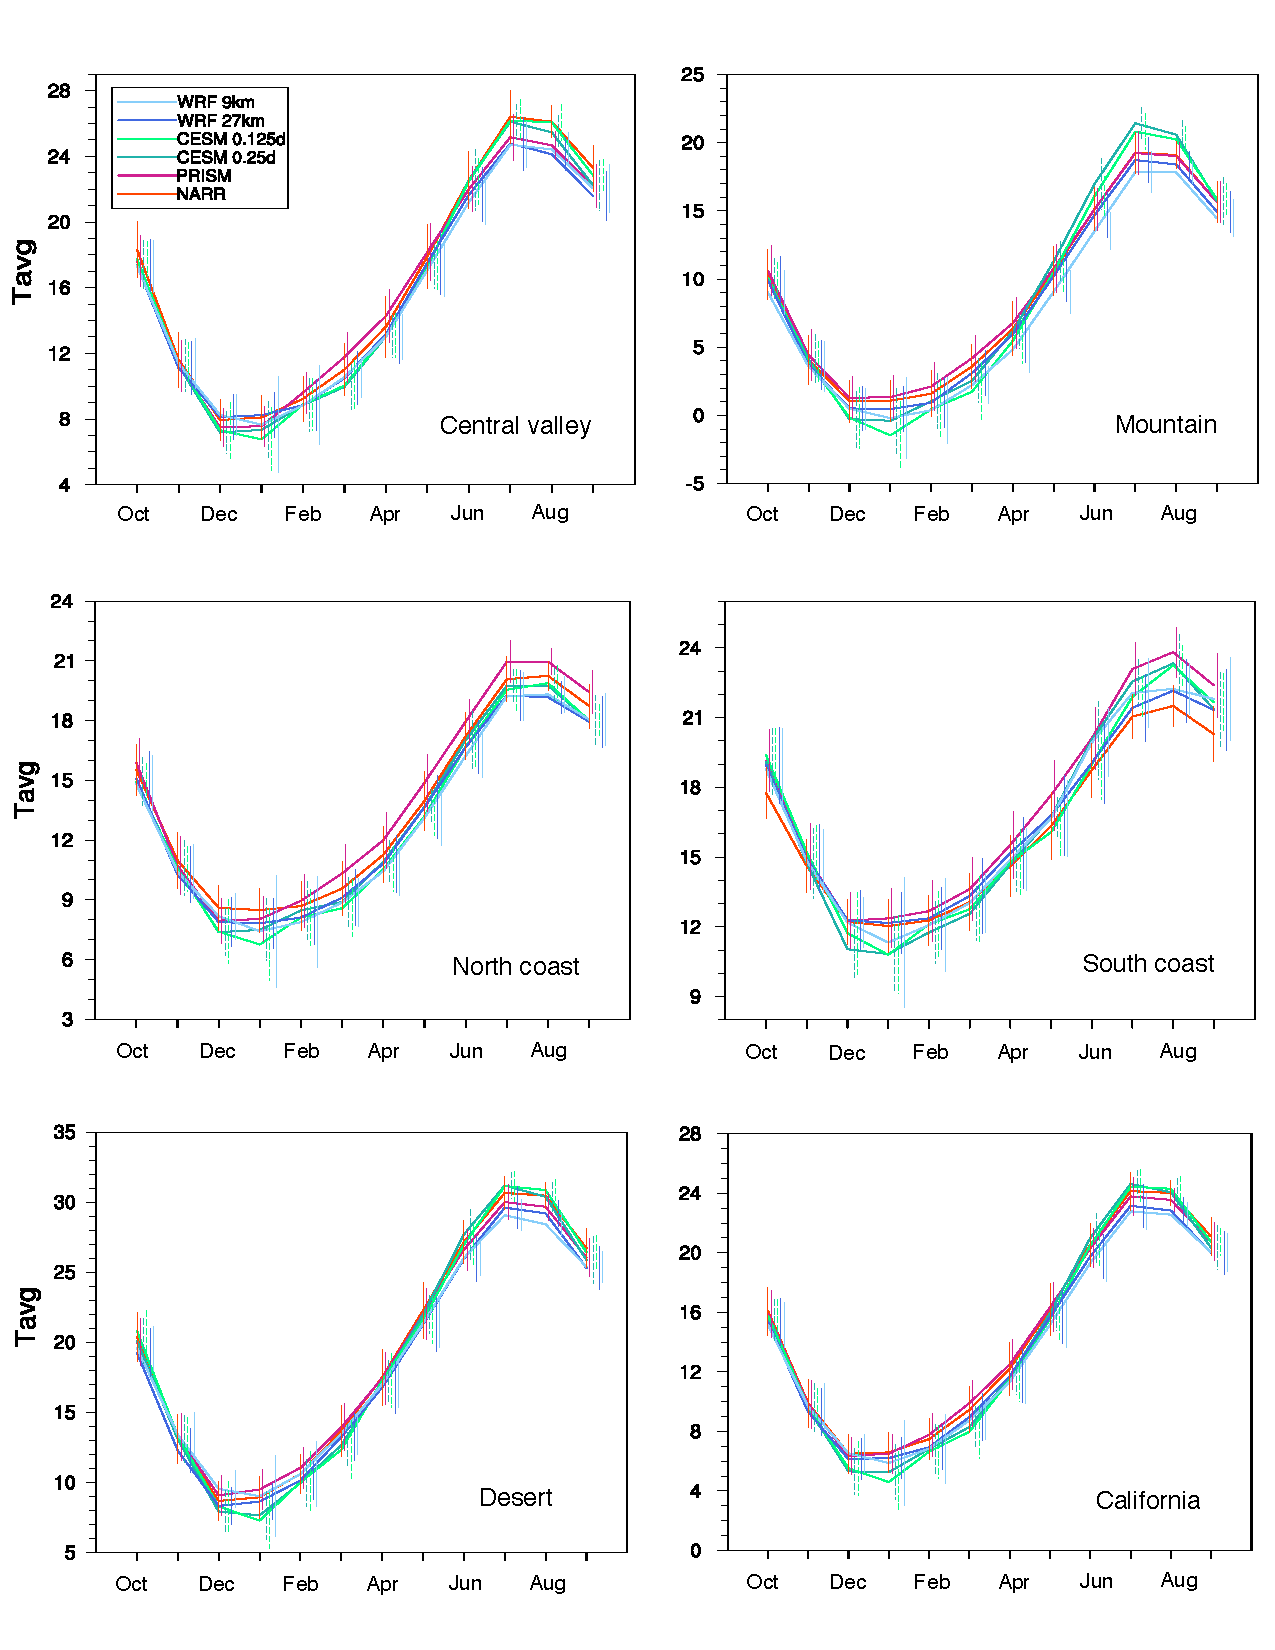
\includegraphics[width=6in]{trd_t2_allzones.pdf}
\end{center}
\caption{Seasonal cycle of monthly-average Tavg for each subzone ($^\circ C$). Bars represent standard deviation ($\sigma$) values.} \label{fig:trd_t2_allzones}
\end{figure}

\begin{figure}
\begin{center}
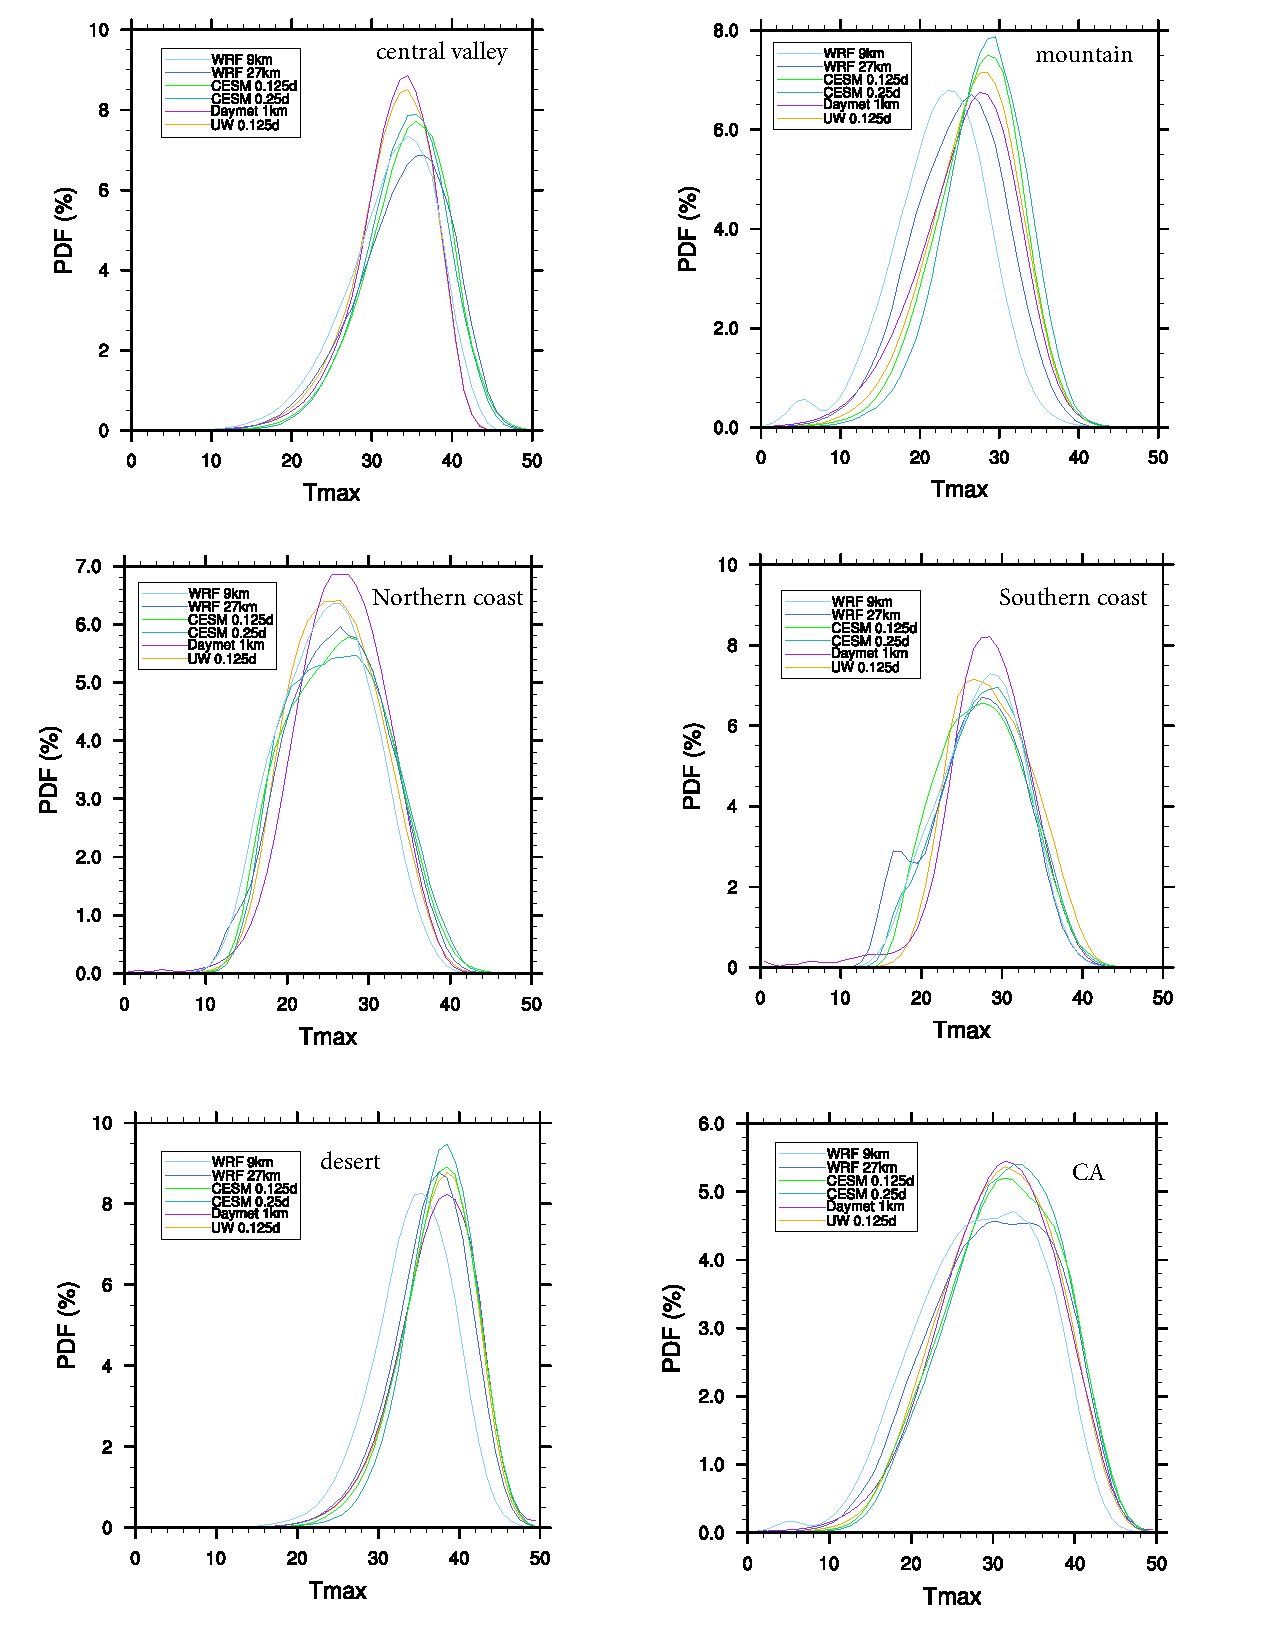
\includegraphics[width=6in]{PDF_t2max_allzones_JJA.pdf}
\end{center}
\caption{Frequency distribution of summer Tmax ($^\circ C$).} \label{fig:PDF_t2max_allzones_JJA}
\end{figure}

%\begin{figure}
%\begin{center}
%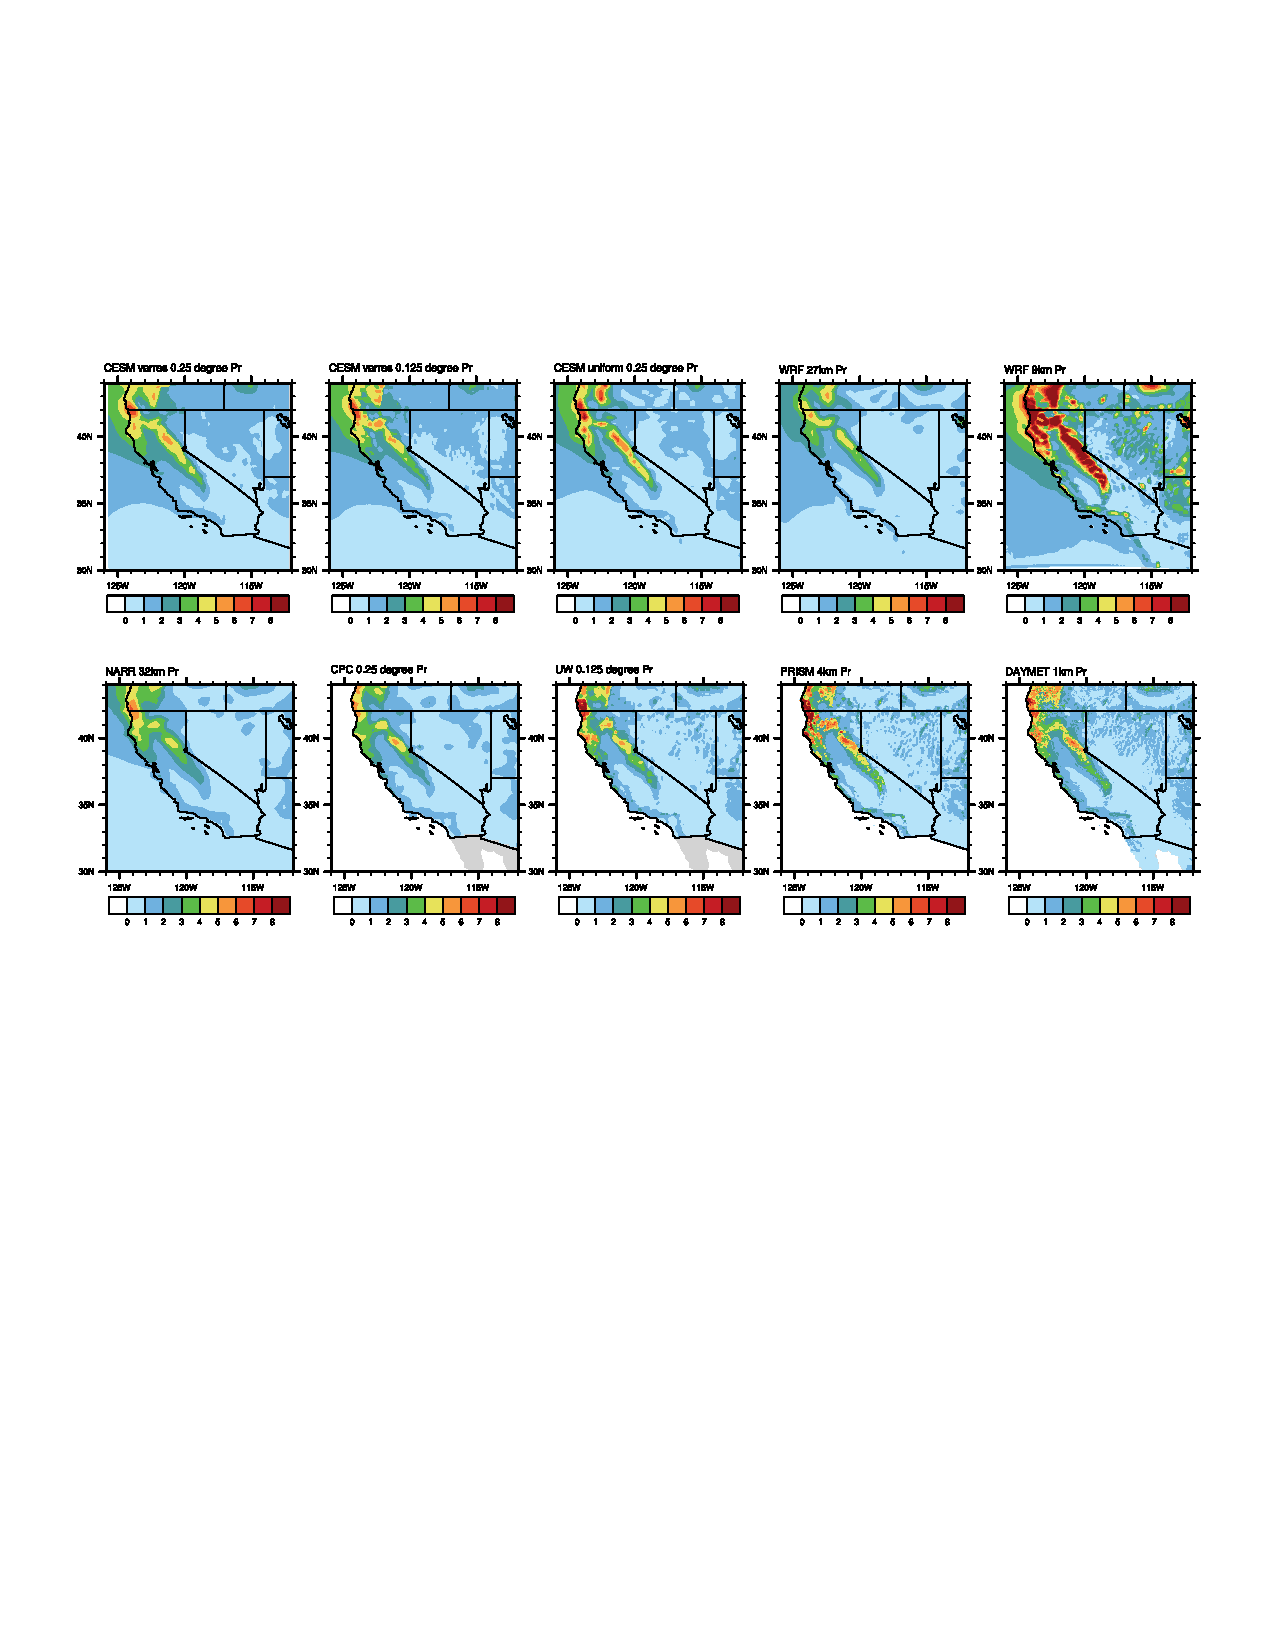
\includegraphics[width=6in]{pr.pdf}
%\end{center}
%\caption{Annual average daily total precipitation from models and reference datasets (mm/d).} \label{fig:Figure11}
%\end{figure}

%relative difference or absolute???

\begin{figure}
\begin{center}
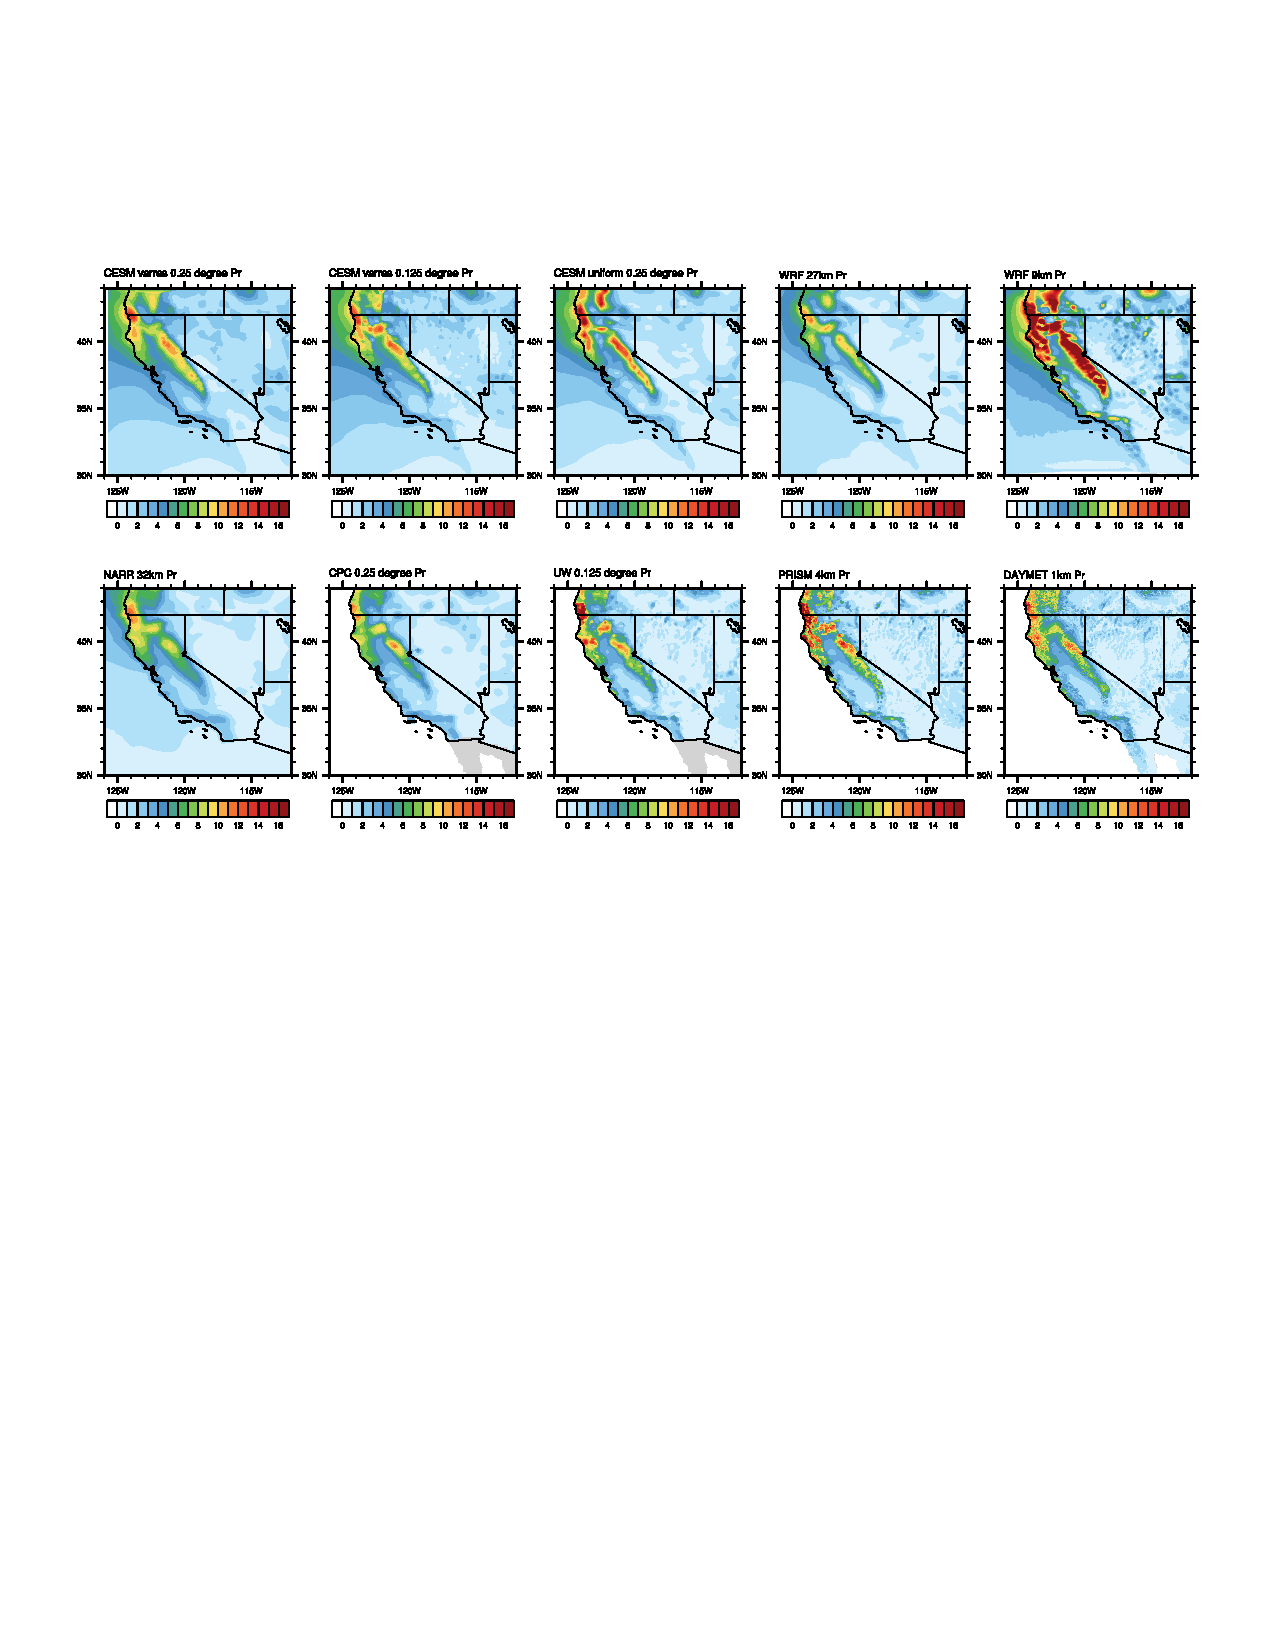
\includegraphics[width=6in]{pr_DJF.pdf}
\end{center}
\caption{Annual DJF precipitation from models and reference datasets (mm/d).} \label{fig:pr_DJF}
\end{figure}

\begin{figure}
\begin{center}
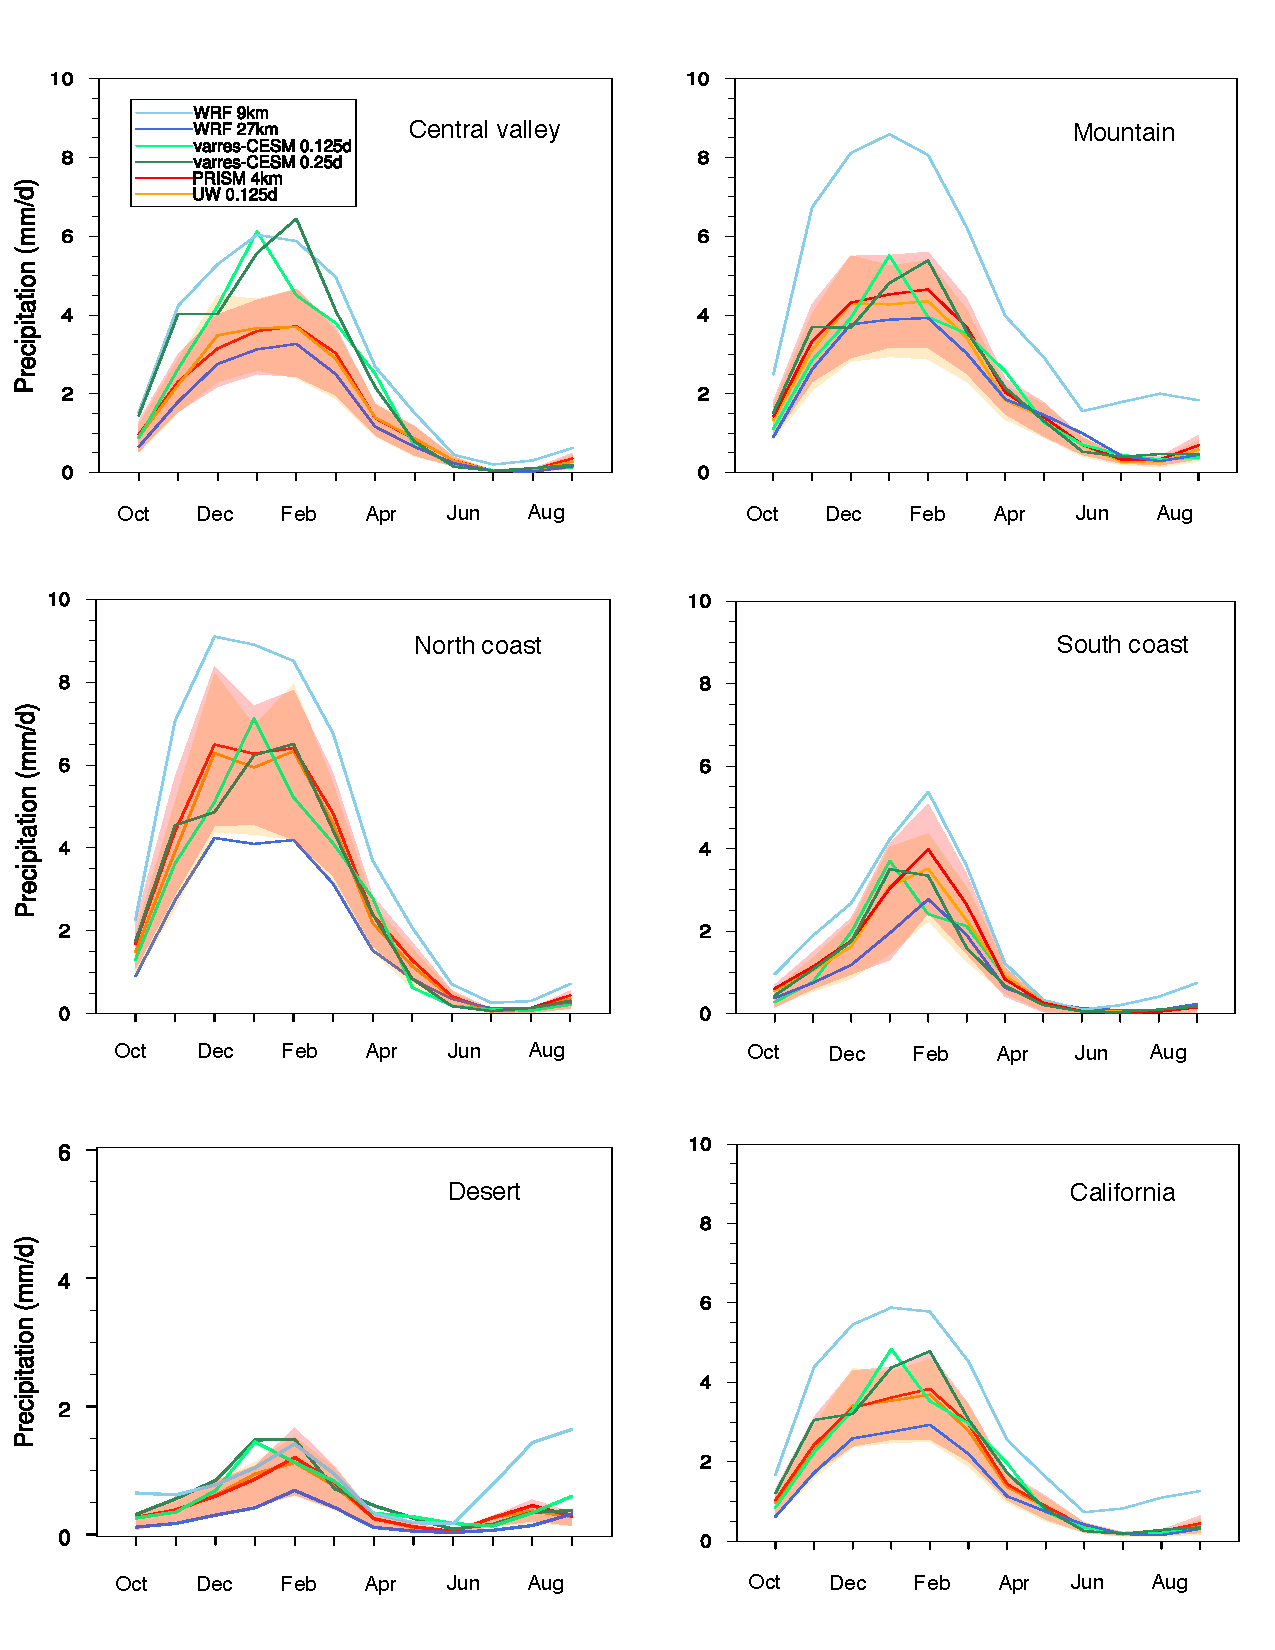
\includegraphics[width=6in]{trd_pr_allzones.pdf}
\end{center}
\caption{As Figure 9, but for monthly-average total precipitation (mm/d).} \label{fig:trd_pr_allzones}
\end{figure}

%CPC is close to NARR for most regions, did not use these two here

\begin{figure}
\begin{center}
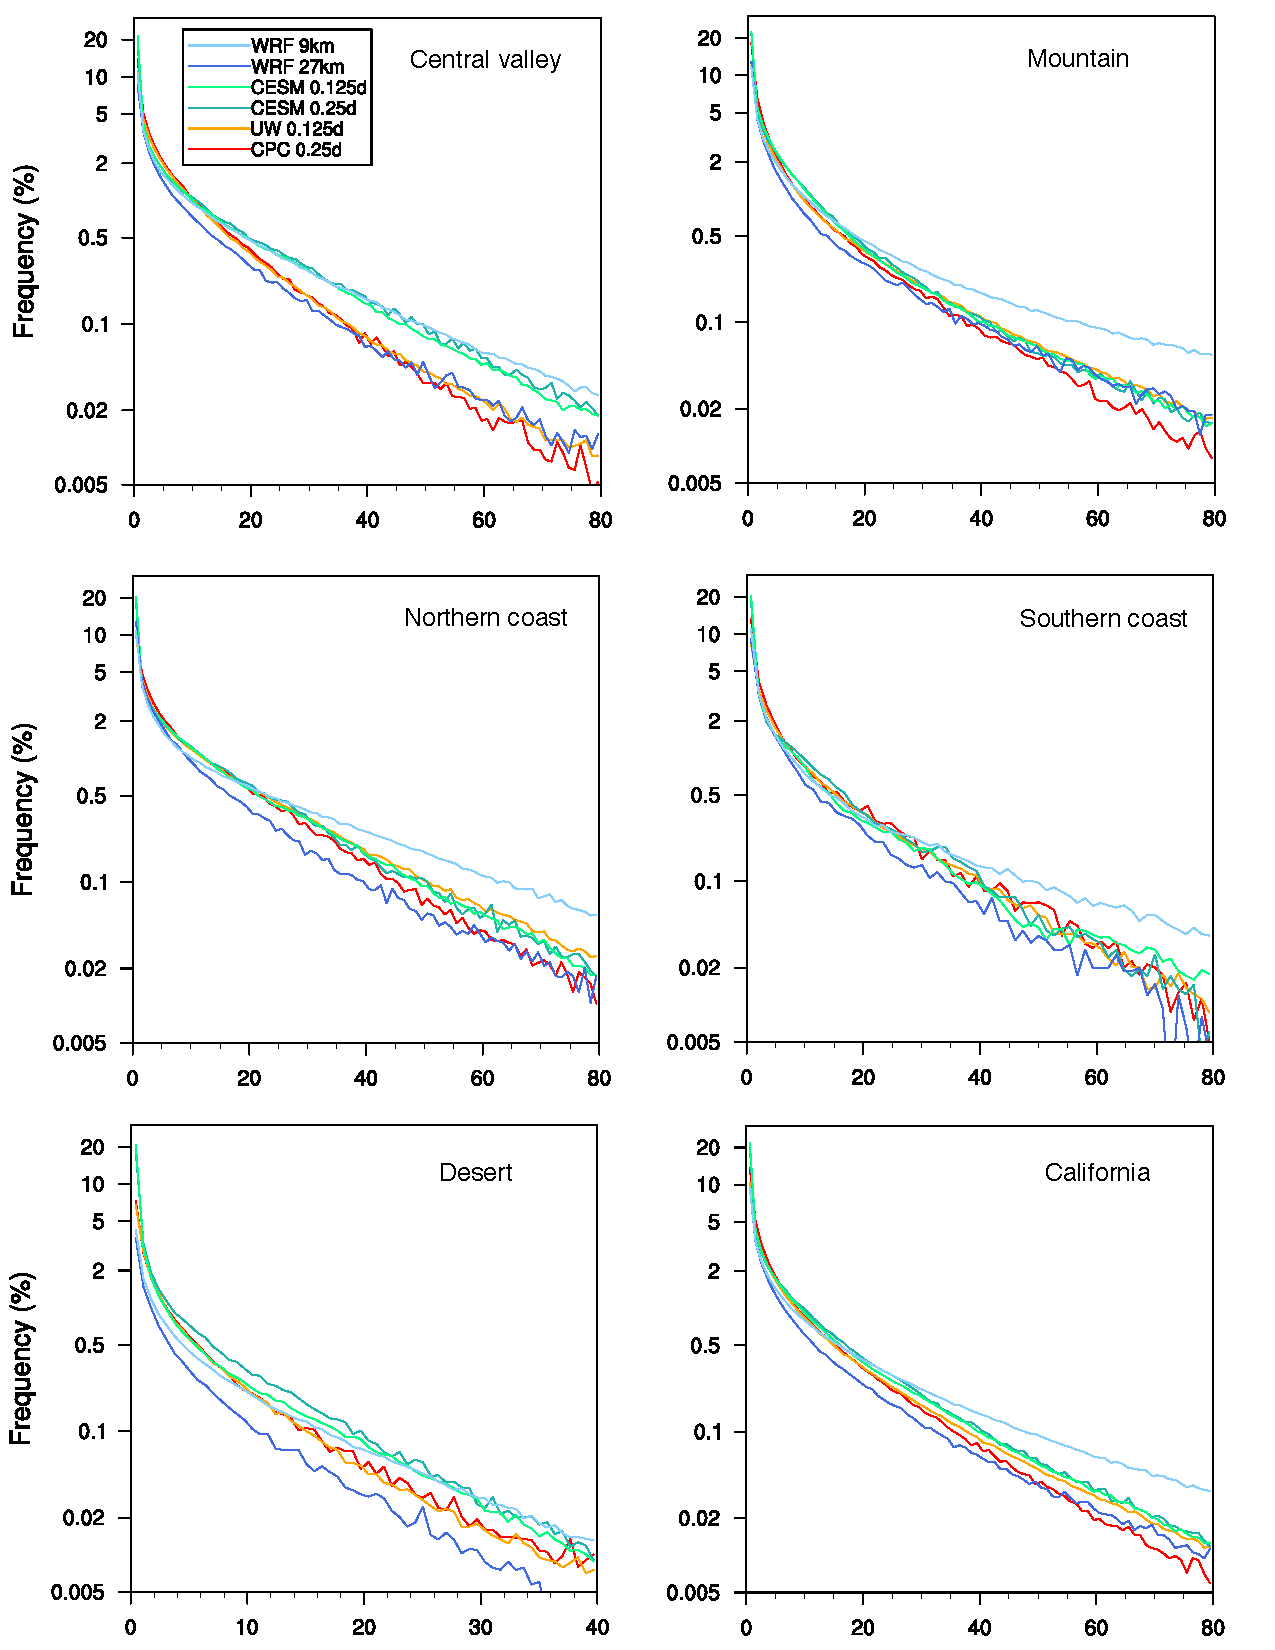
\includegraphics[width=6in]{PDF_pr_allzones_DJF.pdf}
\end{center}
\caption{Frequency distribution of winter Pr constructed from 26 years of daily data (mm/d) (note that the vertical scale is logarithmic).} \label{fig:PDF_pr_allzones_DJF}
\end{figure}

\begin{figure}
\begin{center}
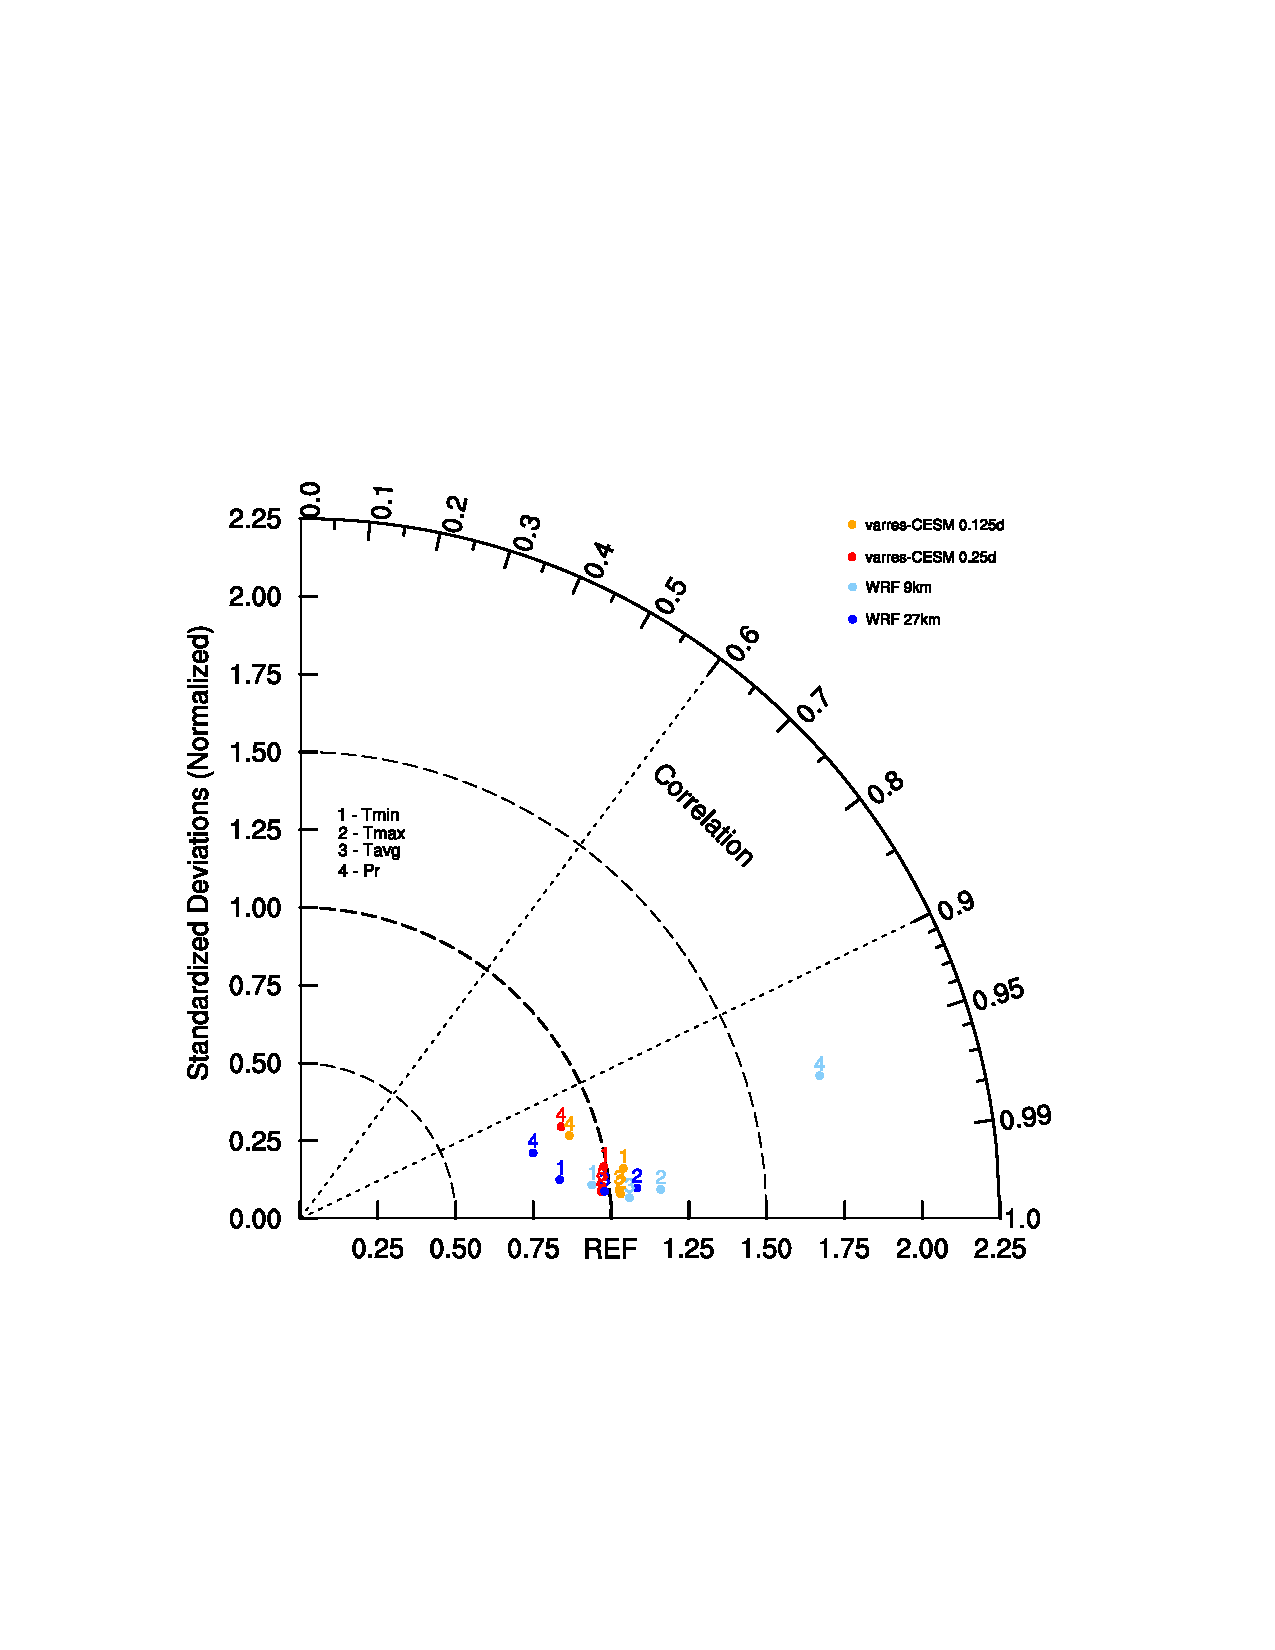
\includegraphics[width=6in]{taylor_diagram.pdf}
\end{center}
\caption{Taylor diagram of annual climatology for the entire California region, using the PRISM dataset as reference.} \label{fig:taylor_diagram}
\end{figure}

\begin{figure}
\begin{center}
\includegraphics[width=6in]{vr_uni_CESM.pdf}
\end{center}
\caption{Comparison of simulated climatology between varres-CESM 0.25 degree and uniform CESM-FV 0.25 degree.} \label{fig:vr_uni_CESM}
\end{figure}


%%%%%%%other notes%%%%%%%%%%%%%%%%%%%
%ERA-Interim is a global atmospheric reanalysis from 1979, continuously updated in real time. The spatial resolution of the data set is approximately 80 km with 60 vertical levels from the surface up to 0.1 hPa (http://www.ecmwf.int/en/research/climate-reanalysis/era-interim). The simulation started at 0000UTC 1 January 1979 and ended at 2400 UTC 31 December 2005 for 27 years. The first year was treated as model spin-up. 10 grid points are used as lateral relaxation zones.

%As for the shortwave and longwave radiation schemes, based on former studies, CAM scheme of the NCAR Community Atmospheric model (Collins et al. 2004), and Rapid Radiation Transfer Model long-wave radiation (Mlawer et al. 1997) and Dudhia short-wave radiation (Dudhia 1989) are tested. As for the cumulus scheme, Kain-Fritsch (new Eta) scheme and Grell-Freitas ensemble scheme are both tested.

%Table for test modeling
%	Model 1	Model 2	Model 3	Model 4	Model 5 (without nudging)
%Radiation scheme	CAM scheme for shortwave and longwave	CAM scheme for shortwave and longwave	Duhia scheme, RRTM scheme	Duhia scheme, RRTM scheme	Duhia scheme, RRTM scheme
%Cumulus scheme	KF scheme	GF scheme	KF scheme	GF scheme	KF scheme

%CESM: This framework has been under development for nearly two decades, and has been used heavily in better understanding the effects of global climate change. The spectral element method has several important properties including parallel scalability, exibility and accuracy, that make it a desirable choice for modeling atmospheric dynamics. The spectral element dynamical core (Fournier et al., 2004; Taylor and Fournier, 2010) is now the default dynamical core in CAM and so is a supported platform for scientific research. which allows for coupled climate simulations in CAM on a variable resolution atmospheric mesh. 

%varres-CESM: Both atmospheric grids are coupled to ocean/ice and land models through the CPL7 tri-grid coupler (Craig et al. 2012), which allows fluxes passed between the atmosphere and other model components to be conservatively remapped to the different grids. We utilize the Community Land Model (CLM) version 4.0 which is run on a 0.9 by 1.25? latitude-longitude grid. The land model is not prescribed and freely adjusts with the climate system. 

%%CAM5 is the newest set of physical parameterizations available within CESM and has been shown to be the superior choice within CAM for variable-resolution simulations due to improved scaling of cloud fraction and precipitation at multiple resolutions when compared to prior versions (Zarzycki et al. 2014b).

%A description of the CESM framework has recently been provided by Hurrell et al. (2013). 

%%%%%%%%%%%%%%%%%%%%%%%%%%%%%%%%%%%%%%%%%%%%%%%%%%%%%%%%%%%%%%%%%%%%%
% END OF AMSPAPER.TEX
%%%%%%%%%%%%%%%%%%%%%%%%%%%%%%%%%%%%%%%%%%%%%%%%%%%%%%%%%%%%%%%%%%%%%

\end{document}
